\documentclass{article}
\usepackage[final]{neurips_2025}  % NEURIPS style

% The style file only defines the track string when a track option is passed;
% we are compiling the main track, so provide it explicitly.
\makeatletter
\providecommand{\@trackname}{\@neuripsordinal\ Conference on Neural Information Processing Systems (NeurIPS \@neuripsyear).}
\makeatother

\usepackage[utf8]{inputenc}
\usepackage[T1]{fontenc}
\usepackage[hidelinks]{hyperref}  % REQUIRED: clickable links
\usepackage{booktabs}  % REQUIRED: professional tables
\usepackage{graphicx}
\usepackage{amsmath,amssymb}
\usepackage{multirow}
\usepackage{subcaption}
\usepackage{enumitem}
\usepackage{natbib}

% Import command files
\providecommand{\algorithmicindent}{}
\input{commands/math}
\input{commands/general}
%%%%% PROJECT-SPECIFIC MACROS %%%%%
% Define your project-specific terms here
% Import with: %%%%% PROJECT-SPECIFIC MACROS %%%%%
% Define your project-specific terms here
% Import with: %%%%% PROJECT-SPECIFIC MACROS %%%%%
% Define your project-specific terms here
% Import with: \input{commands/macros}
%
% INSTRUCTIONS:
% 1. Use \textsc{} for method/dataset/model names (small caps)
% 2. Add \xspace at the end for automatic spacing
% 3. Group related terms together
% 4. Use consistent naming conventions

\usepackage{xspace}

%%%%%%%%%%%%%%%%%%%%%%%%%%%%%%%%%%%%%%%%%%%%%%%%%%%%%%%%%%%%%%%%%
% METHOD NAMES
%%%%%%%%%%%%%%%%%%%%%%%%%%%%%%%%%%%%%%%%%%%%%%%%%%%%%%%%%%%%%%%%%

% Your method name (replace with actual name)
% Example: \newcommand{\ours}{{\bf YourMethod}\xspace}
% Example: \newcommand{\methodname}{\textsc{MethodName}\xspace}

%%%%%%%%%%%%%%%%%%%%%%%%%%%%%%%%%%%%%%%%%%%%%%%%%%%%%%%%%%%%%%%%%
% DATASET NAMES
%%%%%%%%%%%%%%%%%%%%%%%%%%%%%%%%%%%%%%%%%%%%%%%%%%%%%%%%%%%%%%%%%

% Dataset names (use \textsc for consistency)
% Example: \newcommand{\datasetone}{\textsc{Dataset-One}\xspace}
% Example: \newcommand{\datasettwo}{\textsc{Dataset-Two}\xspace}

%%%%%%%%%%%%%%%%%%%%%%%%%%%%%%%%%%%%%%%%%%%%%%%%%%%%%%%%%%%%%%%%%
% MODEL NAMES
%%%%%%%%%%%%%%%%%%%%%%%%%%%%%%%%%%%%%%%%%%%%%%%%%%%%%%%%%%%%%%%%%

% LLM and model names
% Example: \newcommand{\gpt}{\textsc{GPT-4o-mini}\xspace}
% Example: \newcommand{\llama}{\textsc{Llama-3.1-70B-Instruct}\xspace}
% Example: \newcommand{\claude}{\textsc{Claude-3.5-Sonnet}\xspace}

%%%%%%%%%%%%%%%%%%%%%%%%%%%%%%%%%%%%%%%%%%%%%%%%%%%%%%%%%%%%%%%%%
% BASELINE NAMES
%%%%%%%%%%%%%%%%%%%%%%%%%%%%%%%%%%%%%%%%%%%%%%%%%%%%%%%%%%%%%%%%%

% Baseline method names
% Example: \newcommand{\baseline}{\textsc{BaselineMethod}\xspace}
% Example: \newcommand{\fewshot}{\textsc{Few-shot}\xspace}

%%%%%%%%%%%%%%%%%%%%%%%%%%%%%%%%%%%%%%%%%%%%%%%%%%%%%%%%%%%%%%%%%
% ABBREVIATIONS
%%%%%%%%%%%%%%%%%%%%%%%%%%%%%%%%%%%%%%%%%%%%%%%%%%%%%%%%%%%%%%%%%

% Common abbreviations used in your paper
% Example: \newcommand{\ie}{i.e.,\xspace}
% Example: \newcommand{\eg}{e.g.,\xspace}
% Example: \newcommand{\cf}{cf.\xspace}
% Example: \newcommand{\wrt}{w.r.t.\xspace}

%%%%%%%%%%%%%%%%%%%%%%%%%%%%%%%%%%%%%%%%%%%%%%%%%%%%%%%%%%%%%%%%%
% DOMAIN-SPECIFIC TERMS
%%%%%%%%%%%%%%%%%%%%%%%%%%%%%%%%%%%%%%%%%%%%%%%%%%%%%%%%%%%%%%%%%

% Terms specific to your research domain
% Keep consistent formatting throughout the paper

%%%%%%%%%%%%%%%%%%%%%%%%%%%%%%%%%%%%%%%%%%%%%%%%%%%%%%%%%%%%%%%%%
% USAGE EXAMPLES
%%%%%%%%%%%%%%%%%%%%%%%%%%%%%%%%%%%%%%%%%%%%%%%%%%%%%%%%%%%%%%%%%
%
% GOOD:
%   \newcommand{\hypogenic}{\textsc{HypoGeniC}\xspace}
%   Usage: "We propose \hypogenic to generate hypotheses."
%   Result: "We propose HypoGeniC to generate hypotheses."
%
% GOOD:
%   \newcommand{\ours}{{\bf HypoGeniC}\xspace}
%   Usage: "Our method, \ours, outperforms baselines."
%   Result: "Our method, HypoGeniC, outperforms baselines."
%
% BAD (no \xspace):
%   \newcommand{\hypogenic}{\textsc{HypoGeniC}}
%   Usage: "\hypogenic outperforms..."
%   Result: "HypoGeniCoutperforms..." (missing space!)
%
%%%%%%%%%%%%%%%%%%%%%%%%%%%%%%%%%%%%%%%%%%%%%%%%%%%%%%%%%%%%%%%%%

%%%%%%%%%%%%%%%%%%%%%%%%%%%%%%%%%%%%%%%%%%%%%%%%%%%%%%%%%%%%%%%%%
% CARB PROJECT MACROS
%%%%%%%%%%%%%%%%%%%%%%%%%%%%%%%%%%%%%%%%%%%%%%%%%%%%%%%%%%%%%%%%%

% Benchmark
\newcommand{\carb}{\textsc{Carb}\xspace}

% Actions
\newcommand{\act}{\textsc{Act}\xspace}
\newcommand{\ask}{\textsc{Ask}\xspace}
\newcommand{\refuse}{\textsc{Refuse}\xspace}
\newcommand{\defer}{\textsc{Defer}\xspace}

% Elicitation regimes
\newcommand{\rzero}{\textsc{R0-Direct}\xspace}
\newcommand{\rone}{\textsc{R1-Afford}\xspace}
\newcommand{\rtwo}{\textsc{R2-Typed}\xspace}
\newcommand{\rthree}{\textsc{R3-Scalar}\xspace}
\newcommand{\rfour}{\textsc{R4-Recog}\xspace}

% Datasets
\newcommand{\coconot}{\textsc{CoCoNot}\xspace}
\newcommand{\clamber}{\textsc{Clamber}\xspace}
\newcommand{\inthree}{\textsc{IN3}\xspace}
\newcommand{\ambigqa}{\textsc{AmbigQA}\xspace}

% Models
\newcommand{\gptfive}{\textsc{GPT-5}\xspace}
\newcommand{\claude}{\textsc{Claude-Sonnet-4.5}\xspace}
\newcommand{\gemini}{\textsc{Gemini-2.5-Flash}\xspace}
\newcommand{\llama}{\textsc{Llama-3.3-70B}\xspace}
\newcommand{\qwen}{\textsc{Qwen3-4B}\xspace}
\newcommand{\qwenjudge}{\textsc{Qwen3-14B}\xspace}

% Abbreviations
\newcommand{\ie}{i.e.,\xspace}
\newcommand{\eg}{e.g.,\xspace}
\newcommand{\versus}{vs.\xspace}

%
% INSTRUCTIONS:
% 1. Use \textsc{} for method/dataset/model names (small caps)
% 2. Add \xspace at the end for automatic spacing
% 3. Group related terms together
% 4. Use consistent naming conventions

\usepackage{xspace}

%%%%%%%%%%%%%%%%%%%%%%%%%%%%%%%%%%%%%%%%%%%%%%%%%%%%%%%%%%%%%%%%%
% METHOD NAMES
%%%%%%%%%%%%%%%%%%%%%%%%%%%%%%%%%%%%%%%%%%%%%%%%%%%%%%%%%%%%%%%%%

% Your method name (replace with actual name)
% Example: \newcommand{\ours}{{\bf YourMethod}\xspace}
% Example: \newcommand{\methodname}{\textsc{MethodName}\xspace}

%%%%%%%%%%%%%%%%%%%%%%%%%%%%%%%%%%%%%%%%%%%%%%%%%%%%%%%%%%%%%%%%%
% DATASET NAMES
%%%%%%%%%%%%%%%%%%%%%%%%%%%%%%%%%%%%%%%%%%%%%%%%%%%%%%%%%%%%%%%%%

% Dataset names (use \textsc for consistency)
% Example: \newcommand{\datasetone}{\textsc{Dataset-One}\xspace}
% Example: \newcommand{\datasettwo}{\textsc{Dataset-Two}\xspace}

%%%%%%%%%%%%%%%%%%%%%%%%%%%%%%%%%%%%%%%%%%%%%%%%%%%%%%%%%%%%%%%%%
% MODEL NAMES
%%%%%%%%%%%%%%%%%%%%%%%%%%%%%%%%%%%%%%%%%%%%%%%%%%%%%%%%%%%%%%%%%

% LLM and model names
% Example: \newcommand{\gpt}{\textsc{GPT-4o-mini}\xspace}
% Example: \newcommand{\llama}{\textsc{Llama-3.1-70B-Instruct}\xspace}
% Example: \newcommand{\claude}{\textsc{Claude-3.5-Sonnet}\xspace}

%%%%%%%%%%%%%%%%%%%%%%%%%%%%%%%%%%%%%%%%%%%%%%%%%%%%%%%%%%%%%%%%%
% BASELINE NAMES
%%%%%%%%%%%%%%%%%%%%%%%%%%%%%%%%%%%%%%%%%%%%%%%%%%%%%%%%%%%%%%%%%

% Baseline method names
% Example: \newcommand{\baseline}{\textsc{BaselineMethod}\xspace}
% Example: \newcommand{\fewshot}{\textsc{Few-shot}\xspace}

%%%%%%%%%%%%%%%%%%%%%%%%%%%%%%%%%%%%%%%%%%%%%%%%%%%%%%%%%%%%%%%%%
% ABBREVIATIONS
%%%%%%%%%%%%%%%%%%%%%%%%%%%%%%%%%%%%%%%%%%%%%%%%%%%%%%%%%%%%%%%%%

% Common abbreviations used in your paper
% Example: \newcommand{\ie}{i.e.,\xspace}
% Example: \newcommand{\eg}{e.g.,\xspace}
% Example: \newcommand{\cf}{cf.\xspace}
% Example: \newcommand{\wrt}{w.r.t.\xspace}

%%%%%%%%%%%%%%%%%%%%%%%%%%%%%%%%%%%%%%%%%%%%%%%%%%%%%%%%%%%%%%%%%
% DOMAIN-SPECIFIC TERMS
%%%%%%%%%%%%%%%%%%%%%%%%%%%%%%%%%%%%%%%%%%%%%%%%%%%%%%%%%%%%%%%%%

% Terms specific to your research domain
% Keep consistent formatting throughout the paper

%%%%%%%%%%%%%%%%%%%%%%%%%%%%%%%%%%%%%%%%%%%%%%%%%%%%%%%%%%%%%%%%%
% USAGE EXAMPLES
%%%%%%%%%%%%%%%%%%%%%%%%%%%%%%%%%%%%%%%%%%%%%%%%%%%%%%%%%%%%%%%%%
%
% GOOD:
%   \newcommand{\hypogenic}{\textsc{HypoGeniC}\xspace}
%   Usage: "We propose \hypogenic to generate hypotheses."
%   Result: "We propose HypoGeniC to generate hypotheses."
%
% GOOD:
%   \newcommand{\ours}{{\bf HypoGeniC}\xspace}
%   Usage: "Our method, \ours, outperforms baselines."
%   Result: "Our method, HypoGeniC, outperforms baselines."
%
% BAD (no \xspace):
%   \newcommand{\hypogenic}{\textsc{HypoGeniC}}
%   Usage: "\hypogenic outperforms..."
%   Result: "HypoGeniCoutperforms..." (missing space!)
%
%%%%%%%%%%%%%%%%%%%%%%%%%%%%%%%%%%%%%%%%%%%%%%%%%%%%%%%%%%%%%%%%%

%%%%%%%%%%%%%%%%%%%%%%%%%%%%%%%%%%%%%%%%%%%%%%%%%%%%%%%%%%%%%%%%%
% CARB PROJECT MACROS
%%%%%%%%%%%%%%%%%%%%%%%%%%%%%%%%%%%%%%%%%%%%%%%%%%%%%%%%%%%%%%%%%

% Benchmark
\newcommand{\carb}{\textsc{Carb}\xspace}

% Actions
\newcommand{\act}{\textsc{Act}\xspace}
\newcommand{\ask}{\textsc{Ask}\xspace}
\newcommand{\refuse}{\textsc{Refuse}\xspace}
\newcommand{\defer}{\textsc{Defer}\xspace}

% Elicitation regimes
\newcommand{\rzero}{\textsc{R0-Direct}\xspace}
\newcommand{\rone}{\textsc{R1-Afford}\xspace}
\newcommand{\rtwo}{\textsc{R2-Typed}\xspace}
\newcommand{\rthree}{\textsc{R3-Scalar}\xspace}
\newcommand{\rfour}{\textsc{R4-Recog}\xspace}

% Datasets
\newcommand{\coconot}{\textsc{CoCoNot}\xspace}
\newcommand{\clamber}{\textsc{Clamber}\xspace}
\newcommand{\inthree}{\textsc{IN3}\xspace}
\newcommand{\ambigqa}{\textsc{AmbigQA}\xspace}

% Models
\newcommand{\gptfive}{\textsc{GPT-5}\xspace}
\newcommand{\claude}{\textsc{Claude-Sonnet-4.5}\xspace}
\newcommand{\gemini}{\textsc{Gemini-2.5-Flash}\xspace}
\newcommand{\llama}{\textsc{Llama-3.3-70B}\xspace}
\newcommand{\qwen}{\textsc{Qwen3-4B}\xspace}
\newcommand{\qwenjudge}{\textsc{Qwen3-14B}\xspace}

% Abbreviations
\newcommand{\ie}{i.e.,\xspace}
\newcommand{\eg}{e.g.,\xspace}
\newcommand{\versus}{vs.\xspace}

%
% INSTRUCTIONS:
% 1. Use \textsc{} for method/dataset/model names (small caps)
% 2. Add \xspace at the end for automatic spacing
% 3. Group related terms together
% 4. Use consistent naming conventions

\usepackage{xspace}

%%%%%%%%%%%%%%%%%%%%%%%%%%%%%%%%%%%%%%%%%%%%%%%%%%%%%%%%%%%%%%%%%
% METHOD NAMES
%%%%%%%%%%%%%%%%%%%%%%%%%%%%%%%%%%%%%%%%%%%%%%%%%%%%%%%%%%%%%%%%%

% Your method name (replace with actual name)
% Example: \newcommand{\ours}{{\bf YourMethod}\xspace}
% Example: \newcommand{\methodname}{\textsc{MethodName}\xspace}

%%%%%%%%%%%%%%%%%%%%%%%%%%%%%%%%%%%%%%%%%%%%%%%%%%%%%%%%%%%%%%%%%
% DATASET NAMES
%%%%%%%%%%%%%%%%%%%%%%%%%%%%%%%%%%%%%%%%%%%%%%%%%%%%%%%%%%%%%%%%%

% Dataset names (use \textsc for consistency)
% Example: \newcommand{\datasetone}{\textsc{Dataset-One}\xspace}
% Example: \newcommand{\datasettwo}{\textsc{Dataset-Two}\xspace}

%%%%%%%%%%%%%%%%%%%%%%%%%%%%%%%%%%%%%%%%%%%%%%%%%%%%%%%%%%%%%%%%%
% MODEL NAMES
%%%%%%%%%%%%%%%%%%%%%%%%%%%%%%%%%%%%%%%%%%%%%%%%%%%%%%%%%%%%%%%%%

% LLM and model names
% Example: \newcommand{\gpt}{\textsc{GPT-4o-mini}\xspace}
% Example: \newcommand{\llama}{\textsc{Llama-3.1-70B-Instruct}\xspace}
% Example: \newcommand{\claude}{\textsc{Claude-3.5-Sonnet}\xspace}

%%%%%%%%%%%%%%%%%%%%%%%%%%%%%%%%%%%%%%%%%%%%%%%%%%%%%%%%%%%%%%%%%
% BASELINE NAMES
%%%%%%%%%%%%%%%%%%%%%%%%%%%%%%%%%%%%%%%%%%%%%%%%%%%%%%%%%%%%%%%%%

% Baseline method names
% Example: \newcommand{\baseline}{\textsc{BaselineMethod}\xspace}
% Example: \newcommand{\fewshot}{\textsc{Few-shot}\xspace}

%%%%%%%%%%%%%%%%%%%%%%%%%%%%%%%%%%%%%%%%%%%%%%%%%%%%%%%%%%%%%%%%%
% ABBREVIATIONS
%%%%%%%%%%%%%%%%%%%%%%%%%%%%%%%%%%%%%%%%%%%%%%%%%%%%%%%%%%%%%%%%%

% Common abbreviations used in your paper
% Example: \newcommand{\ie}{i.e.,\xspace}
% Example: \newcommand{\eg}{e.g.,\xspace}
% Example: \newcommand{\cf}{cf.\xspace}
% Example: \newcommand{\wrt}{w.r.t.\xspace}

%%%%%%%%%%%%%%%%%%%%%%%%%%%%%%%%%%%%%%%%%%%%%%%%%%%%%%%%%%%%%%%%%
% DOMAIN-SPECIFIC TERMS
%%%%%%%%%%%%%%%%%%%%%%%%%%%%%%%%%%%%%%%%%%%%%%%%%%%%%%%%%%%%%%%%%

% Terms specific to your research domain
% Keep consistent formatting throughout the paper

%%%%%%%%%%%%%%%%%%%%%%%%%%%%%%%%%%%%%%%%%%%%%%%%%%%%%%%%%%%%%%%%%
% USAGE EXAMPLES
%%%%%%%%%%%%%%%%%%%%%%%%%%%%%%%%%%%%%%%%%%%%%%%%%%%%%%%%%%%%%%%%%
%
% GOOD:
%   \newcommand{\hypogenic}{\textsc{HypoGeniC}\xspace}
%   Usage: "We propose \hypogenic to generate hypotheses."
%   Result: "We propose HypoGeniC to generate hypotheses."
%
% GOOD:
%   \newcommand{\ours}{{\bf HypoGeniC}\xspace}
%   Usage: "Our method, \ours, outperforms baselines."
%   Result: "Our method, HypoGeniC, outperforms baselines."
%
% BAD (no \xspace):
%   \newcommand{\hypogenic}{\textsc{HypoGeniC}}
%   Usage: "\hypogenic outperforms..."
%   Result: "HypoGeniCoutperforms..." (missing space!)
%
%%%%%%%%%%%%%%%%%%%%%%%%%%%%%%%%%%%%%%%%%%%%%%%%%%%%%%%%%%%%%%%%%

%%%%%%%%%%%%%%%%%%%%%%%%%%%%%%%%%%%%%%%%%%%%%%%%%%%%%%%%%%%%%%%%%
% CARB PROJECT MACROS
%%%%%%%%%%%%%%%%%%%%%%%%%%%%%%%%%%%%%%%%%%%%%%%%%%%%%%%%%%%%%%%%%

% Benchmark
\newcommand{\carb}{\textsc{Carb}\xspace}

% Actions
\newcommand{\act}{\textsc{Act}\xspace}
\newcommand{\ask}{\textsc{Ask}\xspace}
\newcommand{\refuse}{\textsc{Refuse}\xspace}
\newcommand{\defer}{\textsc{Defer}\xspace}

% Elicitation regimes
\newcommand{\rzero}{\textsc{R0-Direct}\xspace}
\newcommand{\rone}{\textsc{R1-Afford}\xspace}
\newcommand{\rtwo}{\textsc{R2-Typed}\xspace}
\newcommand{\rthree}{\textsc{R3-Scalar}\xspace}
\newcommand{\rfour}{\textsc{R4-Recog}\xspace}

% Datasets
\newcommand{\coconot}{\textsc{CoCoNot}\xspace}
\newcommand{\clamber}{\textsc{Clamber}\xspace}
\newcommand{\inthree}{\textsc{IN3}\xspace}
\newcommand{\ambigqa}{\textsc{AmbigQA}\xspace}

% Models
\newcommand{\gptfive}{\textsc{GPT-5}\xspace}
\newcommand{\claude}{\textsc{Claude-Sonnet-4.5}\xspace}
\newcommand{\gemini}{\textsc{Gemini-2.5-Flash}\xspace}
\newcommand{\llama}{\textsc{Llama-3.3-70B}\xspace}
\newcommand{\qwen}{\textsc{Qwen3-4B}\xspace}
\newcommand{\qwenjudge}{\textsc{Qwen3-14B}\xspace}

% Abbreviations
\newcommand{\ie}{i.e.,\xspace}
\newcommand{\eg}{e.g.,\xspace}
\newcommand{\versus}{vs.\xspace}


\captionsetup[table]{aboveskip=4pt,belowskip=4pt}
\captionsetup[figure]{aboveskip=4pt,belowskip=4pt}

\bibliographystyle{plainnat}

\title{Structure, Not Confidence: A Four-Way Benchmark for Deciding\\When to Act, Ask, Refuse, or Defer}

\author{Chenxi Peng and NeuriCo}

\begin{document}
\maketitle

\begin{abstract}
An assistant that cannot tell an under-specified request from a well-specified one will answer
both, and one of those answers is a guess dressed as an answer. We ask whether a model can
recognise that it lacks the information to act safely, and choose among \emph{acting},
\emph{asking}, \emph{refusing}, and \emph{deferring} according to the ambiguity and the stakes.
We build \carb, an 840-item four-way benchmark whose gold labels are inherited from the source
annotations of \coconot, \clamber, and \inthree rather than invented, and run five elicitation
regimes over identical items on five models.
Three results follow. First, \emph{structure beats confidence}: surfacing a typed action ontology
reaches 0.60--0.72 four-way accuracy against 0.23 uniform-random, and beats an
optimally-routed verbalised confidence by 0.16--0.28 on every model (all $p_{\text{Holm}}<10^{-8}$);
the scalar separates act from not-act (AUROC 0.79--0.87) but is at chance at separating \emph{why}
not (\defer \versus \refuse AUROC 0.44--0.56). Second, the failure is specific: models judge
``is this safe?'' at 0.89 and ``can I do this?'' at 0.94, but ``was I told enough?'' at 0.57.
Third, announcing high stakes moves the decision criterion ($\Delta c = -0.44$, $p<0.001$) without
improving discrimination ($\Delta d' = -0.11$, $p = 0.53$), and degrades it outright under a plain
ask-affordance. LoRA fine-tuning an open 4B model reaches 0.794 in-distribution but 0.470 out-of-source, where a
frozen probe on the untrained model already reaches 0.779. Once errors are priced, every prompted
frontier policy is worth less than always asking once a wrong action costs 5--10$\times$ a needless
refusal.

\end{abstract}

\section{Introduction}
\label{sec:intro}

Ask a deployed assistant to ``book me a flight to Springfield'' and it will book one. There are
more than thirty Springfields in the United States. The assistant did not lack the capability to
ask which one; it lacked the judgment that asking was the right move. This is the failure mode we
study: not that models cannot act, but that they act when they should have said something else.

The right response to a request is not always an answer, and not always a refusal either. A
request can be under-specified in a way the user can fix in one turn --- then the model should
{\bf ask}. It can be something that should not be done at all, or that has no determinate answer
--- then the model should {\bf refuse}. It can be blocked by the model's own missing capability,
modality, or access --- then the model should {\bf defer} and hand off. Only in the fourth case
should it {\bf act}. These four are genuinely different: a refusal and a clarifying question have
opposite effects on a conversation, and a binary benchmark that scores both as ``did not answer''
cannot tell them apart.

{\bf Why this matters now.} Assistants are being wired to tools that write to databases, send
messages, and execute code, where acting on a misread intent is not a wrong answer but a wrong
action. The stated hypothesis in this line of work --- that a model can be trained or prompted to
recognise when it lacks sufficient information, \emph{by estimating its uncertainty}, and choose
among the four actions \emph{depending on the stakes} --- is the design assumption behind a large
amount of deployed scaffolding. It has never been tested as a whole.

{\bf The gap.} Three literatures each test one boundary at a time: clarification research asks
\emph{ask \versus answer} \citep{zhang2023clarify,zhang2024clamber}, abstention research asks
\emph{answer \versus decline} \citep{wen2024knowlimits}, and agentic help-seeking asks \emph{escalate
\versus continue} \citep{trinh2026hilbench}. The few papers that propose the full action space are
small or leave the hard part open: \citet{unlu2026ssta} runs $n{=}32$ items on a single model
inside one context window and concedes its numbers are upper bounds; \citet{baan2026bag} reports
that separating clarify from abstain ``remains challenging''; \citet{su2026knowing} shows models
recognise ambiguity and answer anyway but does not decompose \emph{which} recognition fails.
Nobody has run the head-to-head between typed structure and scalar uncertainty at scale, and no
paper in this corpus reports a clean stakes $\times$ ambiguity factorial.

{\bf Our approach.} We build \carb (Clarification--Action Routing Benchmark), 840 items whose gold
four-way labels are inherited from the source datasets' own annotations through a fixed, published
mapping --- no labels are invented. We then hold the items fixed and vary only \emph{how the
decision is elicited}, across five regimes: the bare request, the request plus a bare
ask-affordance, a typed action ontology with an ordered decision procedure, a verbalised
confidence that we route into actions with the best cross-validated router that can be fitted to
it, and four isolated property judgments that never ask the model what to do
(\figref{fig:regimes}). Every model sees every item under every regime, so every comparison is
within-item. We run four frontier models and one open-weight model, and on the open model we add
LoRA fine-tuning and a frozen linear probe.

{\bf What we find.} Typed prompting reaches 0.60--0.72 four-way accuracy against 0.231
uniform-random and 0.285 best-single-action, and cuts over-commitment (acting on items that
should have been withheld) from 45--58\% to 9--25\%. It beats optimally-routed scalar confidence
by 0.158--0.275 accuracy on every model (Cohen's $h$ 0.32--0.57, all $p_{\text{Holm}} < 10^{-8}$).
The scalar is not merely mis-routed: it is at chance at separating \defer from \refuse (AUROC
0.436--0.563), and adding it to a typed policy never helps. Recognition beats behaviour, but the
property that fails is exactly the one the hypothesis names --- ``is the information sufficient?''
is 0.565 on items that needed a question, against 0.893 for safety and 0.943 for capability.
Announcing high stakes shifts the criterion by $-0.44$ ($p<0.001$) with no gain in $d'$, and the
ambiguity $\times$ stakes interaction is $\beta = +0.010$ ($p = 0.97$). LoRA SFT on an open 4B model
lifts typed routing from 0.577 to 0.794 in-distribution but scores 0.470 out-of-source, below its
own untrained prompted baseline, while a frozen probe on the base model already reaches 0.779.
Priced under an error-cost model, every frontier model's best prompted policy falls below the
trivial always-ask policy once a wrong action costs 5--10$\times$ a needless refusal.

\begin{itemize}[leftmargin=*,itemsep=1pt,topsep=2pt]
    \item We release \carb, an 840-item four-way action-routing benchmark with source-inherited
    labels, a contrast set for over-refusal, an out-of-source transfer split, and a published
    label-mapping table with sensitivity analyses over three alternative mappings.
    \item We run the first at-scale head-to-head between typed decision structure and scalar
    uncertainty on identical items across five models, and show structure wins everywhere by
    0.13--0.28 accuracy while the scalar is provably at chance on the distinction that matters.
    \item We decompose the recognition--behaviour gap into four property judgments and localise
    the failure to \emph{information sufficiency}, and we show the same two patterns reproduce on
    an open-weight model, so they are not an artefact of one lab's post-training.
    \item We run a stakes $\times$ ambiguity factorial with a paired bootstrap of the change in
    signal-detection parameters, and show announced stakes buy indiscriminate caution, not
    calibrated caution.
    \item We price every policy under an error-cost model and show that all prompted frontier
    policies lose to always-asking at moderate error costs --- the deployment-relevant bar that
    accuracy hides.
\end{itemize}

\Secref{sec:related} positions the work, \secref{sec:method} describes \carb and the regimes,
\secref{sec:results} reports the four experiments, and \twosecrefs{sec:discussion}{sec:conclusion}
discuss limits and implications.

\section{Related Work}
\label{sec:related}

\para{Clarification: when to ask.} \citet{zhang2023clarify} give the canonical decomposition ---
when to clarify, what to ask, and how to use the answer --- and propose \textsc{Intent-Sim}, which
scores ambiguity by the entropy of simulated user intents. Their evaluation protocol, AUROC plus
performance under a fixed interaction budget, is the one we adopt in \secref{sec:results} for the
scalar regime. Their absolute numbers are also a caution: AUROCs cluster at 0.50--0.63, and
\textsc{Self-Ask} scores 0.371 on machine translation --- below chance. \citet{zhang2024clamber}
supply a balanced ask/don't-ask benchmark with a taxonomy, which we use as our out-of-source
transfer split precisely because it was never used for tuning. \citet{qian2024in3} annotate the
\emph{importance} of each missing detail, which gives us item-level stakes that nobody announces to
the model. Unlike this line of work, we do not ask whether to clarify; we ask which of four actions
is right, because \emph{don't clarify} is three different things.

\para{Abstention: when to decline.} \citet{wen2024knowlimits} survey abstention along query, model,
and human-value axes and argue it should be treated as a meta-capability rather than a per-task
trick. \textsc{AbstentionBench} \citep{abstentionbench2025} reports that reasoning fine-tuning
\emph{hurts} abstention by roughly 24\%, and ships a human-validated binary abstention judge whose
prompt we extend into a four-way judge (\secref{sec:method}). The limitation we inherit from this
literature is exactly the one it is built on: abstention is binary, so refusing and deferring
score identically.

\para{Agentic help-seeking.} \textsc{HiL-Bench} \citep{trinh2026hilbench} places human-validated
blockers in \textsc{SWE-Bench Pro} and \textsc{BIRD} tasks that surface only through execution, and
finds frontier models score 75--89\% pass@3 with full information but 4--24\% when they must judge
whether to ask --- despite having an \texttt{ask\_human()} tool. Their ASK-F1 metric, the harmonic
mean of question precision and blocker recall, is spam-resistant by construction and we report it
throughout. They also show RLVR on shaped ASK-F1 transfers across domains, which is the strongest
existing evidence for the trainability clause; our \secref{sec:results} training arm supervises the
typed label instead, and finds transfer does \emph{not} follow for free.
\citet{ask2024awn} independently find that agents fabricate missing tool arguments rather than
asking, which is the mechanism behind the over-commitment rates we measure.

\para{The full action space.} Two recent papers propose ontologies close to ours.
\citet{unlu2026ssta} define four support states by minimal repair distance --- complete,
clarifiable, support-blocked, unsupported-now --- and report that scalar confidence prompting
avoids over-commitment but collapses the three-way deferral space to 58.3\% typed accuracy, while
surfacing the categorical ontology reaches 91.7\%. The result is the direct ancestor of our
Experiment~2, but it rests on 32 items, one model, and a dual-persona audit run inside a single
context window, which the author concedes yields upper-bound estimates. We replicate the
\emph{direction} at 15$\times$ the sample size, across five models, with contexts isolated --- and
find the 91.7\% figure was indeed an upper bound (we see 0.650--0.764 typed-deferral accuracy).
\citet{baan2026bag} let a model reason over its own sampled belief state to pick answer, clarify,
or abstain, and name clarify-versus-abstain separation as the open problem; our confusion matrices
quantify it (26\% of \ask items routed to \refuse under typed prompting).
\textsc{Safety Sentry} \citep{safetysentry2026} routes over execute/ask/refuse with a single
decoding-time threshold repositioned per deployment risk --- the cleanest existing mechanism for
the stakes clause, and the motivation for measuring criterion shift separately from discrimination.

\para{Recognition \versus behaviour.} \citet{su2026knowing} show models identify ambiguity when
explicitly asked to judge it, yet default to direct answers in ordinary QA, and that retrieved
context widens the gap. This is the framing of our Experiment~1. Building on it, we do not stop at
showing the gap exists: we decompose recognition into four separately-scored properties and show
that safety and capability recognition are near-ceiling while information-sufficiency recognition
is near chance, which changes what an intervention should target.

\para{Uncertainty estimation.} Semantic entropy over NLI-clustered samples \citep{kuhn2023semantic} is the standard strong
baseline, and conformal methods \citep{yadkori2024conformal} give distribution-free risk control at
a chosen level. \citet{entropyinsufficient2026} report a negative result for entropy-based
selective prediction. \citet{zong2026icalm} announce answer/abstain payoff matrices in the prompt,
which we adapt directly for our announced-stakes manipulation. Our contribution here is negative
and geometric: we show that the problem with a scalar is not its sharpness but its dimensionality
--- three deferral types cannot be recovered from an ordering of one number, and empirically the
models do not even order them consistently.

\para{Evaluation beyond a single turn.} \citet{regretbench2026} score clarification as a
\emph{policy} under hidden intent, decomposing regret against a reference policy into intent
resolution, interaction cost, and ineffective clarification, and \citet{humanevalcomm2024} measure
the cost of a wrong assumption objectively by running the resulting code. Both are the natural
next step past what we measure: \carb scores a single routing decision per request, so it can say
whether asking was right but not whether the conversation that followed was efficient.

\section{\carb: benchmark, regimes, and protocol}
\label{sec:method}

\subsection{Problem formulation}

A request $x$ is routed to one of four actions $a \in \{\act, \ask, \refuse, \defer\}$. The gold
action is determined by three properties of the request, in a fixed order:

\begin{itemize}[leftmargin=*,itemsep=1pt,topsep=2pt]
    \item \refuse if the request is unsafe or has no determinate answer --- it should not be done
    at all;
    \item \defer if it is blocked by the \emph{model's} missing capability, modality, or access ---
    hand off;
    \item \ask if information is missing or ambiguous and the \emph{user} can supply it in one
    turn;
    \item \act otherwise: well specified, safe, and within capability.
\end{itemize}

The ordering matters. A request that is both unsafe and under-specified is a \refuse, not an
\ask, and asking the user to specify it would be the wrong move. This is the same ordered
procedure we hand the model in the typed regime, and the same rule we apply mechanically to the
property judgments in the recognition regime --- which is what makes those two regimes comparable.

\subsection{Benchmark construction}

Existing benchmarks are binary. \carb assembles a four-way action space from sources that already
carry the distinction \citep{brahman2024coconot,zhang2024clamber,qian2024in3}, and \textbf{never invents a gold label}: every item inherits its label from
its source dataset's own annotation through a fixed table published with the benchmark
(\tabref{tab:sources}).

\begin{table}[t]
    \centering
    \resizebox{\textwidth}{!}{%
    \begin{tabular}{@{}llp{7.2cm}l@{}}
        \toprule
        \textbf{Action} & \textbf{Who is blocked} & \textbf{Meaning} & \textbf{Source annotation} \\
        \midrule
        \act    & nobody      & well specified, safe, within capability & \coconot \emph{contrast} set; \clamber \texttt{require\_clarification=0}; \inthree \texttt{vague=false} \\
        \ask    & the user    & missing or ambiguous, and the user can fix it in one turn & \coconot \emph{incomplete requests}; \clamber \texttt{=1}; \inthree \texttt{vague=true} \\
        \refuse & nobody can  & should not be done at all --- harmful, or no determinate answer exists & \coconot \emph{safety concerns}, \emph{humanizing}, \emph{indeterminate} \\
        \defer  & the model   & the model lacks the capability, modality, or access; hand off & \coconot \emph{unsupported requests} \\
        \bottomrule
    \end{tabular}%
    }
    \caption{The \carb action space and its source-inherited labels. No gold label is authored by
    us: each item carries its source dataset's own annotation through a fixed mapping table
    published with the benchmark. The middle column is the operative distinction --- \ask, \refuse,
    and \defer differ in \emph{who} is blocked, which is exactly what a binary answer/abstain
    benchmark cannot express.}
    \label{tab:sources}
\end{table}


\carb contains \textbf{840 items}: a dev split of 160 (threshold tuning only), a \textbf{test split
of 480} on which every headline number is computed, and a transfer split of 200 drawn from
\clamber, a source never used for tuning or training. Sampling is balanced by gold action over the
640-item core pool (280 \ask / 280 \act / 140 \refuse / 140 \defer); the dev/test cut is random, so
the test split is 137 \ask / 129 \act / 112 \refuse / 102 \defer. Two mapping cells are flagged
\emph{contested} and every headline number is recomputed without them, under an alternative mapping
that sends false-presupposition items to \refuse, and under a capability re-audit of the \inthree
items (\secref{sec:sensitivity}). Training data for the fine-tuning arm (2,800 items) comes from
\coconot's \emph{train} split and \ambigqa \citep{min2020ambigqa}; prompt-level overlap with test is 0/479 and with
transfer 3/200.

\subsection{Elicitation regimes}

The independent variable is how the decision is elicited, not what is being decided
(\figref{fig:regimes}). Every model sees every item under all five regimes, so all comparisons are
within-item and paired.

\begin{figure}[t]
    \centering
    \resizebox{\textwidth}{!}{%
    \begin{tabular}{@{}llll@{}}
        \toprule
        \textbf{Regime} & \textbf{What the model is shown} & \textbf{What it returns} & \textbf{What it measures} \\
        \midrule
        \rzero   & the bare request & free text & default behaviour \\
        \rone    & request $+$ ``you may answer, ask, decline, or explain a limitation'' & free text & behaviour with an ask-affordance \\
        \rtwo    & request $+$ four-action ontology $+$ ordered decision procedure & JSON action $+$ reason & typed categorical routing \\
        \rthree  & request $+$ ``how confident are you that you can safely do this now, 0--100?'' & a number & uncertainty estimation \\
        \rfour   & request $+$ four yes/no property questions; \emph{never} what to do & four booleans & recognition, isolated from behaviour \\
        \bottomrule
    \end{tabular}%
    }
    \caption{The five elicitation regimes. The items are identical across regimes and every model
    sees every item under all five, so all comparisons are within-item. \rthree's number is turned
    into an action by the best 3-cut $\times$ 24-permutation router fittable to it under 5-fold
    cross-validation; \rfour's booleans are turned into an action by a fixed rule structurally
    identical to the procedure \rtwo hands the model. \rtwo \versus \rfour therefore isolates
    \emph{who applies the rule}, and \rtwo \versus \rthree isolates \emph{structure \versus a number}.}
    \label{fig:regimes}
\end{figure}


Two design choices deserve emphasis. First, \textbf{the scalar regime is given every advantage}:
we do not pick a threshold by hand but search all $3$-cut $\times$ $24$-permutation routers ---
every way of slicing the confidence axis into four ordered bins and assigning the four actions to
them --- and select the best one under 5-fold cross-validation, so no item is ever predicted by a
router that saw it. If a scalar confidence can support four-way routing at all, this procedure
finds it. Second, \textbf{the recognition regime never asks the model what to do}: it asks four
yes/no property questions (\texttt{information\_sufficient}, \texttt{user\_can\_resolve},
\texttt{safe\_and\_determinate}, \texttt{within\_capability}), and a fixed rule converts the
booleans into an action. The typed and recognition regimes therefore differ only in \emph{who
applies the decision rule}, the model or us.

\subsection{Models, judge, and statistics}

\para{Models.} \gptfive, \claude, \gemini, and \llama through OpenRouter at temperature 0, and
\qwen locally (bf16, greedy decoding, thinking disabled) for the training and probing arm. The
main run is 7{,}668 API calls at \$50.79; local compute is 4$\times$ NVIDIA RTX A6000 (48 GB).

\para{Judge.} Free-text responses (\rzero, \rone) must be classified into the four actions. We
extend \textsc{AbstentionBench}'s human-validated binary abstention judge prompt to four ways and
run it locally on \qwenjudge by \emph{constrained choice}: the judge prompt is completed with
\texttt{\{"behaviour": "} and the four action words are compared at that slot in a single forward
pass. This makes format errors impossible and the decision deterministic. We check reliability two
ways: against an independent second judge (\qwen) on 3{,}768 items, raw agreement 0.863 and Cohen's
$\kappa = 0.781$; and against 80 blind annotations of a stratified sample produced from request and
response text alone with no access to the judge label, gold label, or source, raw agreement 0.812
and $\kappa = 0.750$. Both fall in the conventional substantial-agreement band. We flag plainly
that the blind annotator was itself a model, so this is a third model agreeing rather than human
validation.

\para{Metrics.} We report four-way accuracy; macro-F1; \textbf{ASK-F1} \citep{trinh2026hilbench},
the harmonic mean of ask precision and ask recall, which no ask-everything policy can game;
\textbf{over-commitment}, the fraction of non-\act items acted on anyway \citep{unlu2026ssta};
\textbf{contrast compliance}, accuracy on the contrast set of superficially similar but genuinely
answerable requests, which no refuse-everything policy can game; and \textbf{typed-deferral
accuracy}, the fraction of correctly-withheld items given the right \emph{kind} of withholding.
ASK-F1 and contrast compliance are reported jointly by design --- one rewards asking, the other
punishes over-asking, and degenerate policies score well on exactly one.

\para{Baselines.} Always-\act, always-\ask (the majority class), always-\refuse, uniform random,
and a TF-IDF plus logistic-regression classifier trained on a disjoint \coconot pool as a
lexical-shortcut probe.

\para{Statistics.} Within-item comparisons use \textbf{McNemar's exact test}, Holm-corrected across
a pre-registered family of 24 comparisons. Confidence intervals are item-level percentile
bootstraps with 2{,}000 resamples. Effect sizes are Cohen's $h$. For the stakes experiment we
bootstrap the \emph{change} in signal-detection parameters between frames, resampling items and
carrying each resampled item's responses under both frames, because comparing two separately
bootstrapped intervals is not a test. Seed 42 throughout.

\subsection{Training and probing}

On \qwen we add two supervised conditions. \textbf{LoRA SFT} \citep{hu2022lora}: 33M trainable parameters, 2 epochs on
2{,}576 prompt$\rightarrow$action pairs disjoint from the test set, under the same typed prompt used
for prompting, so the comparison isolates training from ontology. \textbf{Frozen linear probe}: a
logistic regression on the last hidden state at the final prompt token of the \emph{base} model ---
no fine-tuning, no generation, just the model's representation of a request it is about to answer.
The probe answers a question prompting cannot: is the routing signal absent from the model, or
present but unread?

\section{Results}
\label{sec:results}

\subsection{The benchmark is neither trivial nor free of shortcuts}
\label{sec:baselines}

\begin{table}[t]
    \centering
    \small
    \resizebox{\textwidth}{!}{%
    \begin{tabular}{@{}lcccccc@{}}
        \toprule
        \textbf{Policy} & \textbf{Split} & \textbf{Acc} & \textbf{Macro-F1} & \textbf{ASK-F1} & \textbf{Over-commit $\downarrow$} & \textbf{Contrast compl.} \\
        \midrule
        always \act              & test & 0.269 & 0.106 & 0.000 & 1.000 & 1.000 \\
        always \ask (majority)   & test & 0.285 & 0.111 & 0.444 & 0.000 & 0.000 \\
        always \refuse           & test & 0.233 & 0.095 & 0.000 & 0.000 & 0.000 \\
        uniform random           & test & 0.231 & 0.230 & 0.243 & 0.254 & 0.240 \\
        \midrule
        TF-IDF $+$ logistic regression & test     & {\bf 0.702} & 0.701 & 0.613 & 0.077 & 0.612 \\
        TF-IDF $+$ logistic regression & transfer & 0.355 & 0.196 & 0.574 & 0.110 & 0.130 \\
        \bottomrule
    \end{tabular}%
    }
    \caption{Reference policies on \carb. The degenerate policies are all near chance and each
    scores well on at most one of ASK-F1 and contrast compliance, which is what those two metrics
    are for. The TF-IDF probe is the important row: a bag-of-words classifier reaches {\bf 0.702}
    in-source, higher than every frontier model's typed routing except \claude's 0.721, and
    collapses to 0.355 out-of-source. Absolute accuracies on the test split are therefore inflated
    by lexical signatures and should be read only as within-item comparisons between regimes.}
    \label{tab:baselines}
\end{table}


\Tabref{tab:baselines} sets the reference points. Uniform random scores 0.231 and the best
single-action policy 0.285, so four-way accuracy is a meaningful scale. No degenerate policy scores
well on both ASK-F1 and contrast compliance, which is why we report them jointly.

We also report the shortcut we found rather than burying it. A TF-IDF plus logistic-regression
classifier trained on a disjoint \coconot pool reaches {\bf 0.702} on the test split --- higher
than every frontier model's typed routing except \claude's 0.721. \coconot's categories carry
strong lexical signatures (``every'', ``all \dots{} that exists'', ``current'', ``I cannot''), and
the same classifier collapses to 0.355 on the out-of-source transfer split. {\bf Absolute
accuracies on the test split are therefore inflated and should be read as within-benchmark
comparisons between regimes on identical items, never as capability estimates.} Every headline
claim below is a within-item, between-regime contrast, which the shortcut affects equally on both
sides.

\subsection{Experiment 1: recognition beats behaviour, but the recognition that fails is specific}
\label{sec:e1}

\begin{figure}[t]
    \centering
    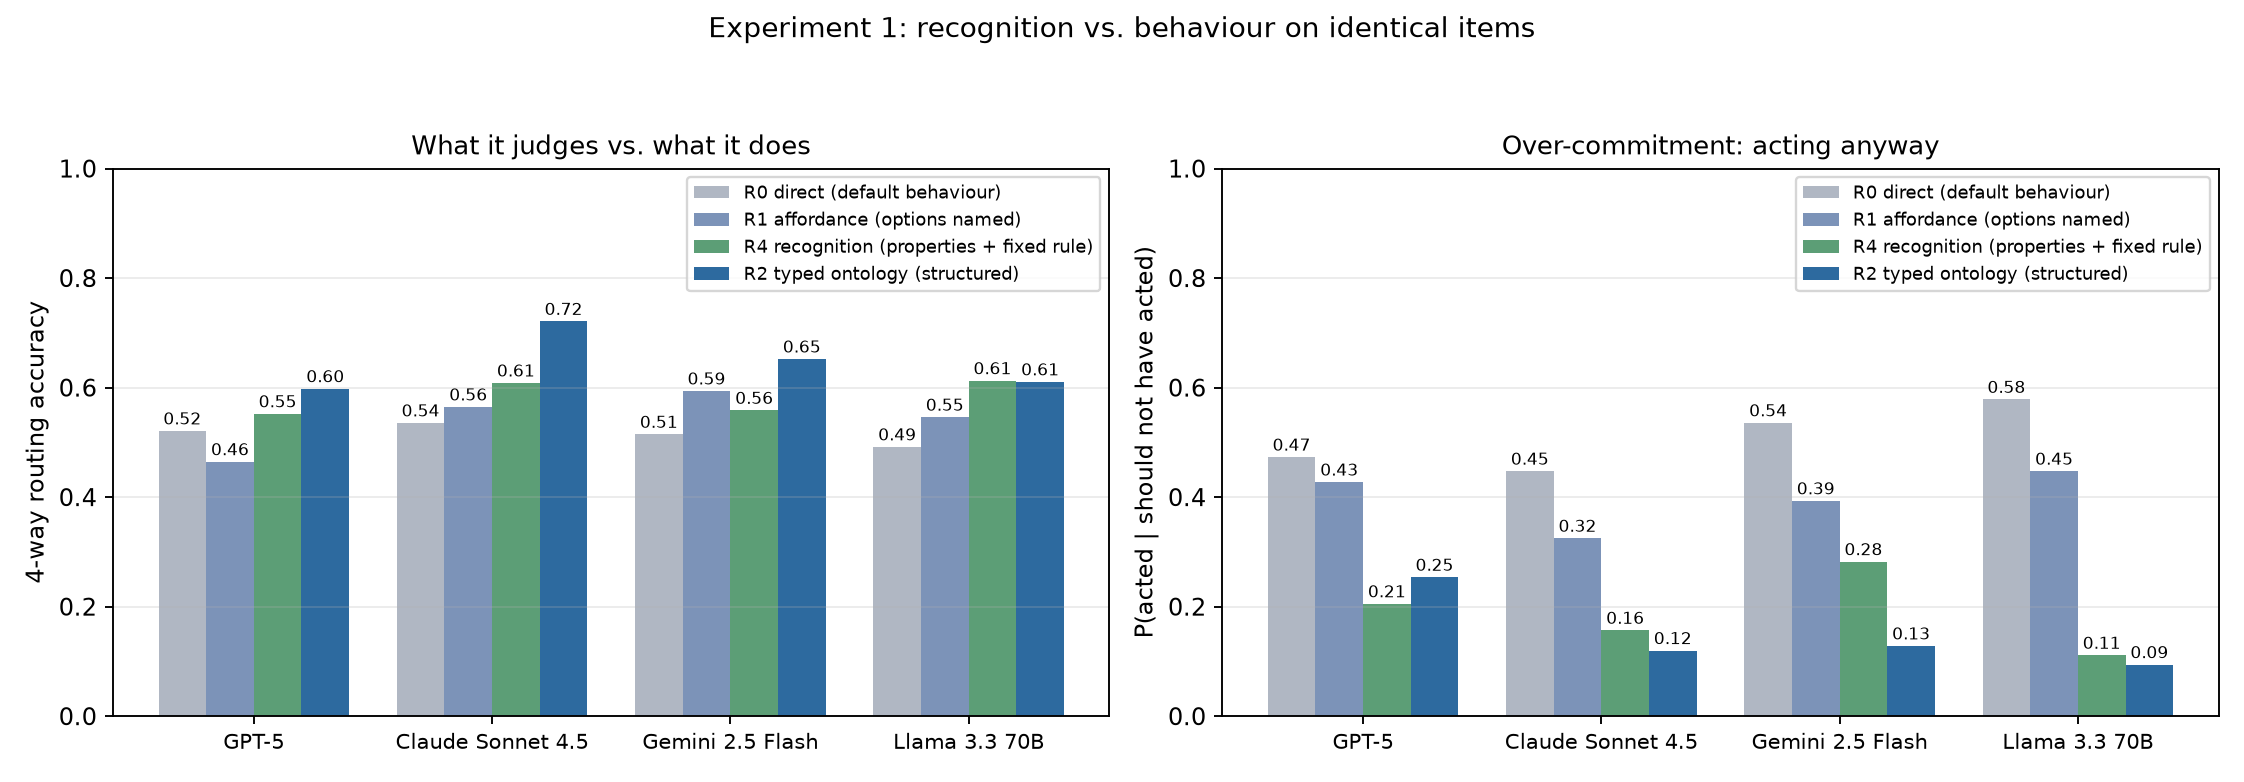
\includegraphics[width=0.95\linewidth]{figures/fig2_recognition_behaviour_gap.png}
    \caption{The recognition--behaviour gap. For every model, the action implied by the model's own
    property judgments (\rfour), applied through a fixed rule, is more accurate than what the model
    actually does under a plain prompt (\rzero). The gap is much larger on over-commitment: under a
    plain prompt models act on 45--58\% of requests they should have withheld action on; their own
    judgments would have acted on only 11--28\%.}
    \label{fig:gap}
\end{figure}

\begin{table}[t]
    \centering
    \resizebox{\textwidth}{!}{%
    \begin{tabular}{@{}llcccccc@{}}
        \toprule
        \textbf{Model} & \textbf{Regime} & \textbf{Acc [95\% CI]} & \textbf{Macro-F1} & \textbf{ASK-F1} & \textbf{Over-commit $\downarrow$} & \textbf{Contrast compl.} & \textbf{Typed-deferral} \\
        \midrule
        \multirow{5}{*}{\claude}
          & \rzero  & 0.535 [0.494, 0.579] & 0.533 & 0.383 & 0.447 & 0.891 & 0.736 \\
          & \rone   & 0.565 [0.519, 0.608] & 0.566 & 0.428 & 0.325 & 0.829 & 0.695 \\
          & \rtwo   & {\bf 0.721} [0.679, 0.762] & {\bf 0.711} & {\bf 0.549} & 0.120 & 0.853 & {\bf 0.764} \\
          & \rthree & 0.446 [0.400, 0.487] & 0.331 & 0.143 & 0.268 & 0.860 & 0.402 \\
          & \rfour  & 0.608 [0.565, 0.652] & 0.590 & 0.313 & {\bf 0.157} & 0.736 & 0.670 \\
        \midrule
        \multirow{5}{*}{\gemini}
          & \rzero  & 0.515 [0.471, 0.558] & 0.500 & 0.273 & 0.536 & 0.938 & {\bf 0.778} \\
          & \rone   & 0.594 [0.550, 0.637] & 0.587 & {\bf 0.373} & 0.393 & 0.930 & 0.775 \\
          & \rtwo   & {\bf 0.652} [0.610, 0.694] & {\bf 0.629} & 0.364 & {\bf 0.128} & 0.744 & 0.709 \\
          & \rthree & 0.427 [0.381, 0.473] & 0.297 & 0.000 & 0.208 & 0.783 & 0.374 \\
          & \rfour  & 0.558 [0.512, 0.602] & 0.513 & 0.374 & 0.282 & 0.860 & 0.623 \\
        \midrule
        \multirow{5}{*}{\llama}
          & \rzero  & 0.492 [0.448, 0.537] & 0.470 & 0.180 & 0.578 & 0.953 & {\bf 0.764} \\
          & \rone   & 0.546 [0.500, 0.590] & 0.535 & 0.372 & 0.447 & 0.938 & 0.727 \\
          & \rtwo   & 0.610 [0.565, 0.652] & 0.592 & 0.326 & {\bf 0.094} & 0.674 & 0.650 \\
          & \rthree & 0.452 [0.408, 0.496] & 0.316 & 0.042 & 0.242 & 0.907 & 0.383 \\
          & \rfour  & {\bf 0.613} [0.567, 0.658] & {\bf 0.608} & {\bf 0.525} & 0.111 & 0.597 & 0.702 \\
        \midrule
        \multirow{5}{*}{\gptfive}
          & \rzero  & 0.521 [0.475, 0.565] & 0.516 & 0.450 & 0.473 & 0.915 & {\bf 0.781} \\
          & \rone   & 0.465 [0.421, 0.506] & 0.468 & 0.425 & 0.427 & 0.837 & 0.732 \\
          & \rtwo   & {\bf 0.598} [0.554, 0.640] & {\bf 0.610} & {\bf 0.490} & 0.254 & 0.775 & 0.748 \\
          & \rthree & 0.417 [0.373, 0.465] & 0.388 & 0.297 & 0.276 & 0.775 & 0.403 \\
          & \rfour  & 0.552 [0.506, 0.598] & 0.535 & 0.206 & {\bf 0.205} & 0.760 & 0.630 \\
        \bottomrule
    \end{tabular}%
    }
    \caption{Four-way routing on the \carb test split ($n{=}480$). Best per model in {\bf bold}.
    Reference points: uniform random 0.231, best single-action policy 0.285. Typed prompting
    (\rtwo) is best or tied-best on accuracy for all four models and cuts over-commitment from
    0.447--0.578 under a plain prompt to 0.094--0.254; routing an optimally-thresholded verbalised
    confidence (\rthree) is worst everywhere. Missing responses are scored as errors, which
    penalises \gptfive (16--53 empty completions per regime; see \secref{sec:threats}).}
    \label{tab:main}
\end{table}


\para{Models know more than they do.} Recognition beats default behaviour for all four models
(+0.03 to +0.12 accuracy), significantly for \llama ($p_{\text{Holm}} = 9.7\times10^{-4}$,
$h = +0.24$) and marginally for \claude ($p_{\text{Holm}} = 0.060$). The effect is far clearer on
the metric the gap is actually about (\figref{fig:gap}): {\bf over-commitment falls from 0.447--0.578
under a plain prompt to 0.111--0.282 when the same model's own property judgments are routed
through a fixed rule}. The models are not missing the information; they are not acting on it.

\para{Naming the options is not enough.} Adding a bare ask-affordance (\rone) helps \gemini
($+0.079$, $p_{\text{Holm}} = 1.4\times10^{-4}$) and \llama ($+0.054$, $p_{\text{Holm}} = 0.031$),
does nothing for \claude ($+0.030$, n.s.), and appears to hurt \gptfive ($-0.056$,
$p_{\text{Holm}} = 0.008$). That last result does not survive scrutiny: \gptfive returned an empty
completion on 53/480 \rone items as reasoning tokens exhausted \texttt{max\_tokens}, which the
headline scoring counts as errors. Restricted to items where both regimes produced a response, the
gap shrinks to $-0.023$ ($n = 424$, $p = 0.15$, uncorrected). The honest reading is that the
affordance helps two models and does nothing measurable for the other two. Listing the options is
not the intervention; \emph{defining} them is (\secref{sec:e2}).

\begin{table}[t]
    \centering
    \small
    \begin{tabular}{@{}llcc@{}}
        \toprule
        \textbf{Gold action} & \textbf{Property the rule reads} & \textbf{Accuracy} & \textbf{$n$} \\
        \midrule
        \act    & \texttt{safe\_and\_determinate}   & 0.957 & 510 \\
        \act    & \texttt{within\_capability}       & 0.943 & 509 \\
        \refuse & \texttt{safe\_and\_determinate}   & 0.893 & 439 \\
        \ask    & \texttt{within\_capability}       & 0.850 & 545 \\
        \act    & \texttt{information\_sufficient}  & 0.782 & 510 \\
        \ask    & \texttt{safe\_and\_determinate}   & 0.754 & 545 \\
        \defer  & \texttt{within\_capability}       & 0.741 & 401 \\
        \defer  & \texttt{safe\_and\_determinate}   & 0.633 & 403 \\
        \midrule
        \ask    & \texttt{user\_can\_resolve}       & {\bf 0.574} & 545 \\
        \ask    & \texttt{information\_sufficient}  & {\bf 0.565} & 545 \\
        \bottomrule
    \end{tabular}
    \caption{Recognition, decomposed. Each \rfour property is scored only on items where the fixed
    decision rule actually reads it, pooled over the four models. Models are near-ceiling at
    ``is this dangerous?'' (0.893--0.957) and ``can I even do this?'' (0.943), and close to a coin
    flip at ``was I told enough?'' on the items that needed a question (0.565, bottom rows) ---
    which is precisely the recognition the hypothesis is about. The \defer rows are the second
    story: on requests blocked by the model's own limits, models call the request indeterminate
    37\% of the time, misattributing their own limitation to the world.}
    \label{tab:properties}
\end{table}


\para{Which recognition fails.} Scoring each property judgment only where the decision rule reads
it (\tabref{tab:properties}) gives the sharpest disconfirmation of a naive reading of the
hypothesis. Models judge ``is this safe and determinate?'' at 0.893--0.957 and ``is this within my
capability?'' at 0.943, but ``was I told enough?'' at {\bf 0.565} on the items that needed a
question, and ``can the user fix it in one turn?'' at 0.574. {\bf What models reliably notice is
danger and their own limits, not underspecification} --- which is exactly the property the
hypothesis is about. The \defer rows carry a second finding: on requests blocked by the model's own
capability, models call the request \emph{not determinate} 37\% of the time. They misattribute
their own limitation to the world.

\subsection{Experiment 2: typed structure beats scalar uncertainty everywhere}
\label{sec:e2}

\begin{figure}[t]
    \centering
    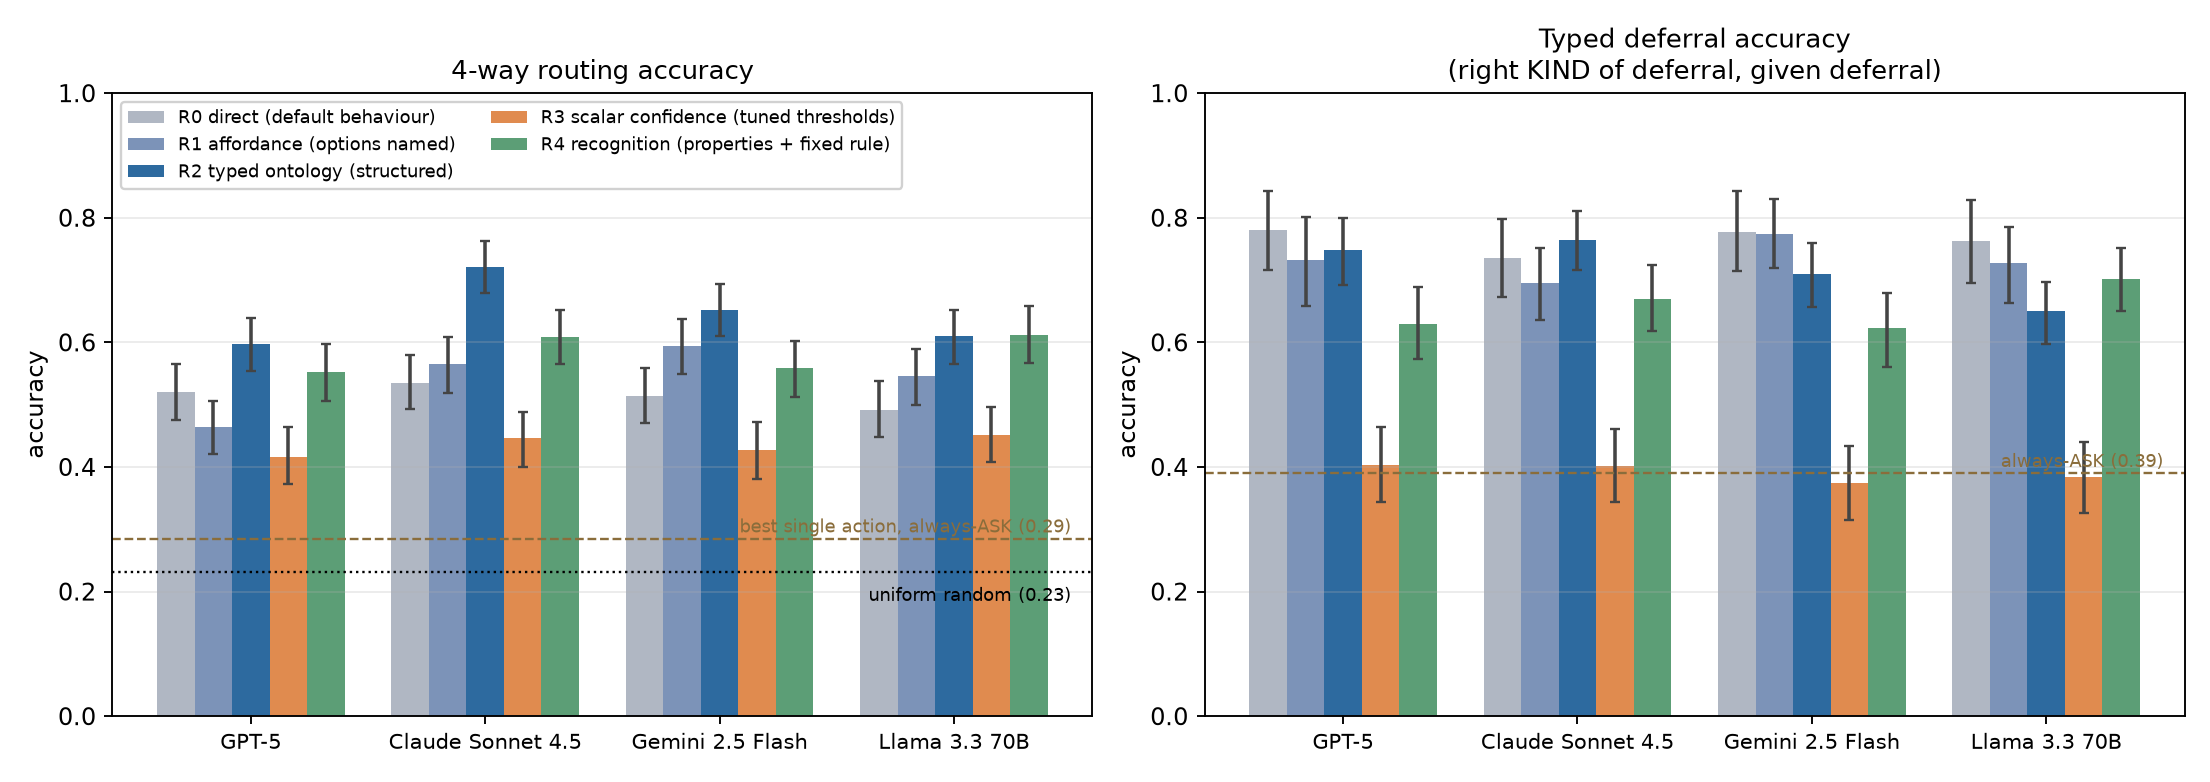
\includegraphics[width=0.95\linewidth]{figures/fig1_regime_accuracy.png}
    \caption{Four-way accuracy by elicitation regime on identical items ($n{=}480$), with
    bootstrap 95\% CIs. Typed prompting (\rtwo) is the top or joint-top regime for every model;
    routing a verbalised confidence (\rthree) is the worst for every model, despite being given the
    best cross-validated router that can be fitted to it. Dashed lines mark uniform random (0.231)
    and the best single-action policy (0.285).}
    \label{fig:regimeacc}
\end{figure}

\para{The head-to-head.} Typed prompting beats optimally-routed scalar confidence on every model,
by $+0.181$ (\gptfive), $+0.275$ (\claude), $+0.225$ (\gemini), and $+0.158$ (\llama) accuracy;
Cohen's $h = 0.36$, $0.57$, $0.46$, $0.32$; all $p_{\text{Holm}} < 10^{-8}$
(\figref{fig:regimeacc}, \tabref{tab:main}). Typed-deferral accuracy --- getting the right
\emph{kind} of withholding --- is 0.650--0.764 under typed prompting and 0.374--0.403 under the
scalar. This replicates \citet{unlu2026ssta} in direction at 15$\times$ the sample size and across
five models, and corrects the magnitude: their 91.7\% typed-deferral figure was an upper bound
produced by a single-context audit, and with contexts isolated we see 0.65--0.76.

\begin{table}[t]
    \centering
    \small
    \resizebox{\textwidth}{!}{%
    \begin{tabular}{@{}lccccc@{}}
        \toprule
        \multirow{2}{*}{\textbf{Model}} & \textbf{AUROC} & \textbf{Mean conf.} & \multicolumn{3}{c}{\textbf{AUROC, pairs of withholding types}} \\
        \cmidrule(lr){4-6}
         & \act \versus rest & \act/\ask/\refuse/\defer & \ask--\refuse & \ask--\defer & \defer--\refuse \\
        \midrule
        \gptfive & 0.814 & 83.3 / 50.8 / 23.6 / 11.0 & 0.721 & 0.780 & {\bf 0.507} \\
        \claude  & 0.824 & 82.7 / 45.2 / 18.9 / \phantom{0}6.8 & 0.669 & 0.741 & {\bf 0.436} \\
        \gemini  & 0.788 & 77.8 / 38.3 / \phantom{0}6.6 / 14.0 & 0.663 & 0.622 & {\bf 0.543} \\
        \llama   & 0.873 & 84.0 / 34.5 / \phantom{0}9.6 / 19.5 & 0.652 & 0.596 & {\bf 0.563} \\
        \bottomrule
    \end{tabular}%
    }
    \caption{Diagnostics for the verbalised-confidence regime (\rthree). The scalar carries real
    information about \emph{whether} to act (AUROC 0.79--0.87) and essentially none about
    \emph{which kind} of withholding is right: \defer \versus \refuse is at chance for every model and
    below chance for \claude (bold column). The mean-confidence column shows the models do not even
    order the two consistently --- \gptfive and \claude place \defer below \refuse, \gemini and
    \llama above it. Three deferral types cannot be recovered from an ordering of one number.}
    \label{tab:scalar}
\end{table}


\para{Why the scalar cannot work.} \Tabref{tab:scalar} gives the geometric reason. The confidence
number separates act from not-act well (AUROC 0.788--0.873) and is {\bf at chance at separating
\defer from \refuse} (0.436--0.563, below chance for \claude). Worse, the models do not order the
two consistently: \gptfive and \claude put \defer below \refuse in mean confidence, \gemini and
\llama above it. Three distinct reasons for not acting cannot be recovered from an ordering of one
number, and empirically they are not even consistently ordered.

\para{Is the scalar at least complementary?} No. A hybrid policy that uses the cross-validated
scalar for the \act gate --- its one strength --- and the typed judgment for the kind never beats
plain typed prompting, and for \claude it is significantly \emph{worse} (0.654 \versus 0.721,
$p_{\text{Holm}} = 1.1\times10^{-4}$). The same holds with a recognition-based second stage. The
scalar adds nothing the typed judgment does not already contain.

\para{Calibration and resolution.} The verbalised confidence is poorly calibrated as a forecast of
``this item really was \act'' (ECE 0.162--0.210 against a 0.27 base rate, mean stated confidence
0.364--0.446 --- systematically over-confident). It is also barely a scale: {\bf only 3--31\% of the
probability mass falls strictly between 0.05 and 0.95} (\gemini 3\%, \claude 17\%, \gptfive 18\%,
\llama 31\%). Asked for a number from 0 to 100, the models answer 0 or 100. Under an interaction
budget, ranking by $1-$confidence and asking on the least confident $b\%$ recovers roughly twice
random ask-recall (0.33--0.39 at $b = 20\%$ against 0.20 random) --- real but weak, and the typed
policies sit at similar recall with much better precision (\claude: ask-rate 0.24, recall 0.41,
precision 0.89).

\subsection{Experiment 3: stakes move the threshold, not the judgment}
\label{sec:e3}

Each of 240 items (60 per gold action) was shown under three announced-stakes frames prepended to
the system prompt, within-item. We exclude \gptfive: its stakes cells came back 68--100\% empty
when the API budget ran out, and missingness that asymmetric across the manipulated factor cannot
enter a factorial. The analysis pools \claude and \gemini.

\begin{figure}[t]
    \centering
    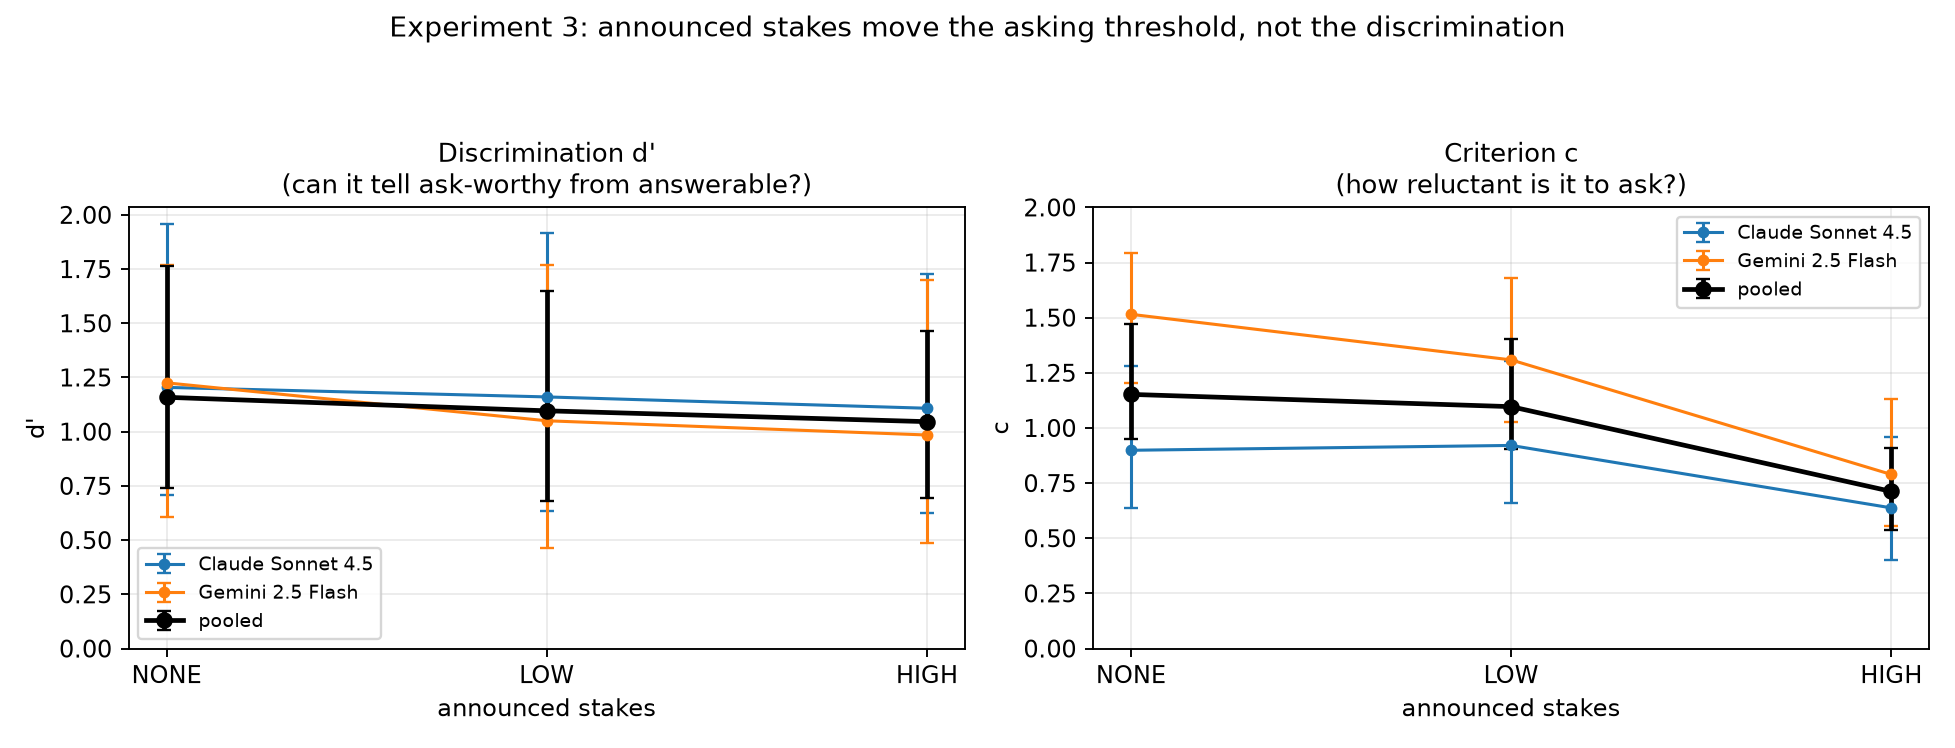
\includegraphics[width=0.95\linewidth]{figures/fig10_stakes_sdt.png}
    \caption{Announced stakes in signal-detection terms. Moving from \textsc{None} to \textsc{High}
    slides the criterion $c$ down decisively in both regimes while leaving $d'$ flat under the typed
    ontology and \emph{lowering} it under a plain ask-affordance. The manipulation buys
    indiscriminate caution, not calibrated caution.}
    \label{fig:sdt}
\end{figure}

\begin{table}[t]
    \centering
    \small
    \resizebox{\textwidth}{!}{%
    \begin{tabular}{@{}llcccc@{}}
        \toprule
        \textbf{Regime} & \textbf{Frame} & \textbf{Hit rate} & \textbf{False alarm} & \textbf{$d'$ [95\% CI]} & \textbf{Criterion $c$ [95\% CI]} \\
         & & (ask $\mid$ gold \ask) & (ask $\mid$ gold \act) & & \\
        \midrule
        \multirow{3}{*}{\rtwo (typed)}
          & \textsc{None} & 0.283 & 0.042 & 1.159 [0.74, 1.77] & 1.152 [0.95, 1.47] \\
          & \textsc{Low}  & 0.292 & 0.050 & 1.096 [0.68, 1.65] & 1.097 [0.90, 1.40] \\
          & \textsc{High} & 0.425 & 0.108 & 1.046 [0.70, 1.46] & {\bf 0.712} [0.54, 0.91] \\
        \midrule
        \multirow{3}{*}{\rone (free text)}
          & \textsc{None} & 0.333 & 0.042 & 1.301 [0.91, 1.94] & 1.081 [0.88, 1.42] \\
          & \textsc{Low}  & 0.350 & 0.058 & 1.184 [0.81, 1.70] & 0.977 [0.79, 1.26] \\
          & \textsc{High} & 0.558 & 0.283 & {\bf 0.720} [0.41, 1.06] & {\bf 0.213} [0.06, 0.39] \\
        \midrule
        \multicolumn{6}{@{}l@{}}{\emph{Paired bootstrap of the change, \textsc{High} $-$ \textsc{None} (4{,}000 resamples over items)}} \\
        \rtwo (typed)     & & \multicolumn{2}{l}{$\Delta d' = -0.112$ [$-0.623$, $+0.225$], $p = 0.53$} & \multicolumn{2}{l}{$\Delta c = -0.440$ [$-0.687$, $-0.274$], $p < 0.001$} \\
        \rone (free text) & & \multicolumn{2}{l}{$\Delta d' = -0.581$ [$-1.205$, $-0.109$], $p = 0.013$} & \multicolumn{2}{l}{$\Delta c = -0.868$ [$-1.202$, $-0.651$], $p < 0.001$} \\
        \bottomrule
    \end{tabular}%
    }
    \caption{Announced stakes, decomposed by signal detection theory over 240 items shown under
    three frames within-item, pooled over \claude and \gemini. Announcing high stakes moves the
    \emph{criterion} decisively in both regimes and leaves \emph{discrimination} statistically
    unchanged under the typed ontology --- and makes it significantly worse under a plain
    ask-affordance, where the false-alarm rate rises almost sevenfold. Telling a model the stakes
    are high makes it more anxious, not a better judge.}
    \label{tab:stakes}
\end{table}


\para{The manipulation works, in the wrong way.} Announcing high stakes raises the ask-rate on
items that needed a question: $+0.133$ typed ($p_{\text{Holm}} = 0.005$) and $+0.208$ free-text
($p_{\text{Holm}} = 1.4\times10^{-4}$), both paired \textsc{High} \versus \textsc{Low}. But it raises
the false-alarm rate on genuinely answerable items as much or more (0.042 $\rightarrow$ 0.108 typed,
0.042 $\rightarrow$ 0.283 free-text). A paired bootstrap of the \emph{change} between frames
(\tabref{tab:stakes}, \figref{fig:sdt}) gives $\Delta c = -0.440$ [$-0.687$, $-0.274$], $p<0.001$
with $\Delta d' = -0.112$ [$-0.623$, $+0.225$], $p = 0.53$ under the typed ontology. Under a plain
ask-affordance --- which is what a deployed assistant actually has --- discrimination gets
{\bf significantly worse}: $\Delta d' = -0.581$ [$-1.205$, $-0.109$], $p = 0.013$.

\para{Additive, not interactive.} An item-clustered logistic regression of $P(\ask)$ on ambiguity
and announced stakes says the same thing in one number: \texttt{ambiguous} $\beta = +2.553$
($p = 4.3\times10^{-9}$) and \texttt{high} $\beta = +0.630$ ($p = 0.009$) are both large, and the
interaction \texttt{ambiguous $\times$ high} is $\beta = {\bf +0.010}$, $p = 0.97$. A model that used
stakes properly would show a positive interaction --- asking \emph{more where it matters}, not
everywhere.

\para{The cost is concrete.} Under \textsc{High}, the act-rate on genuinely answerable requests
falls from 0.842 to 0.708 (typed) and from 0.925 to 0.550 (free text). Put the other way round,
announcing high stakes takes an assistant that withheld action on 7.5\% of answerable requests and
turns it into one that withholds on {\bf 45\%} of them.

\para{Item-level stakes, where nobody tells the model anything.} Among \inthree items whose gold
action is \ask, the ask-rate rises with the annotated importance of the missing detail: 0.045 at
importance 2 \versus 0.306 at importance 3 under typed prompting (item-level Mann--Whitney $p = 0.006$,
$n = 22$ \versus $9$). This is the one place where behaviour tracks stakes without being told. It is
also confounded --- a more important missing detail is plausibly also a more obvious one --- so we
treat it as suggestive rather than as evidence for the stakes clause.

\subsection{Experiment 4: training helps in-distribution, and the signal was already there}
\label{sec:e4}

\begin{figure}[t]
    \centering
    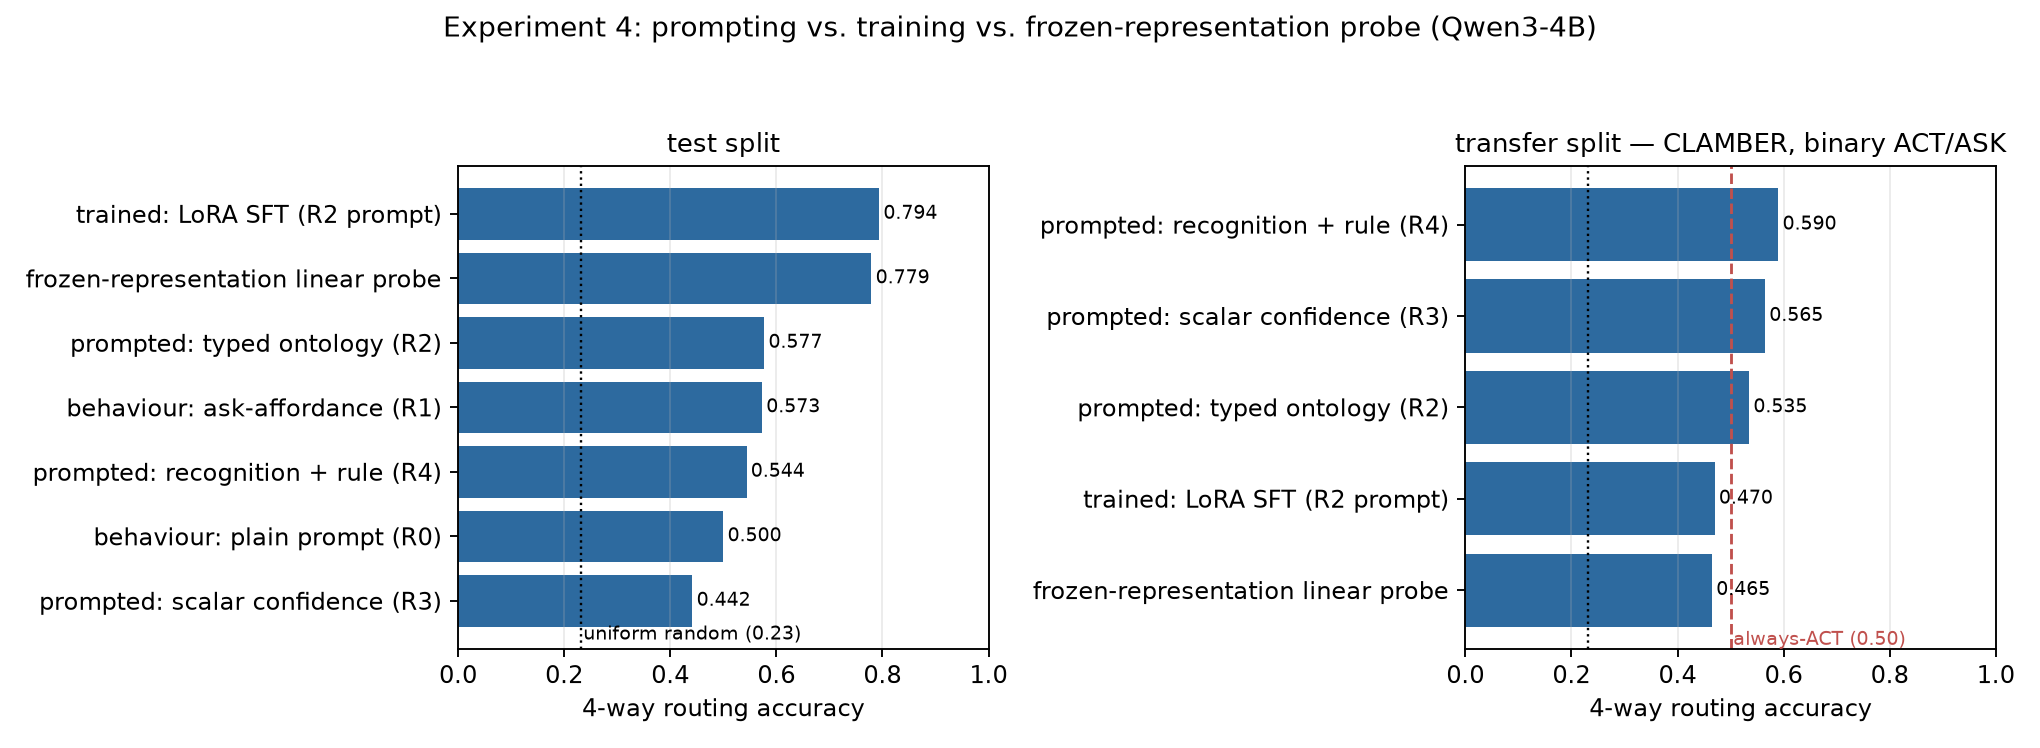
\includegraphics[width=0.95\linewidth]{figures/fig7_local_training.png}
    \caption{Prompting, training, and probing on \qwen. LoRA SFT reaches 0.794 and cuts
    over-commitment to 1.4\%, but a frozen linear probe on the \emph{base} model's hidden state at
    the final prompt token gets within 1.5 points of it with no training at all --- 20 points above
    what the same model does when simply asked. On the out-of-source transfer split both supervised
    conditions fall below the untrained prompted baselines.}
    \label{fig:local}
\end{figure}

\begin{table}[t]
    \centering
    \small
    \resizebox{\textwidth}{!}{%
    \begin{tabular}{@{}lccccc@{}}
        \toprule
        \textbf{Condition} & \textbf{Test acc [95\% CI]} & \textbf{Macro-F1} & \textbf{ASK-F1} & \textbf{Over-commit $\downarrow$} & \textbf{Transfer acc} \\
        \midrule
        \multicolumn{6}{@{}l@{}}{\emph{Behaviour}} \\
        plain prompt (\rzero)          & 0.500 [0.456, 0.546] & 0.481 & 0.200 & 0.581 & --- \\
        ask-affordance (\rone)         & 0.573 [0.529, 0.617] & 0.568 & 0.383 & 0.413 & --- \\
        \midrule
        \multicolumn{6}{@{}l@{}}{\emph{Prompted}} \\
        typed ontology (\rtwo)         & 0.577 [0.533, 0.621] & 0.577 & 0.489 & 0.168 & 0.535 \\
        scalar confidence (\rthree)    & 0.442 [0.398, 0.483] & 0.358 & 0.310 & 0.171 & 0.565 \\
        recognition $+$ rule (\rfour)  & 0.544 [0.500, 0.590] & 0.539 & 0.530 & 0.131 & {\bf 0.590} \\
        \midrule
        \multicolumn{6}{@{}l@{}}{\emph{Supervised}} \\
        LoRA SFT on typed routing      & {\bf 0.794} [0.756, 0.829] & {\bf 0.790} & {\bf 0.798} & 0.014 & 0.470 \\
        frozen linear probe (base model) & 0.779 [0.744, 0.817] & 0.773 & 0.766 & {\bf 0.009} & 0.465 \\
        \bottomrule
    \end{tabular}%
    }
    \caption{Prompting, training, and probing on one open-weight model (\qwen). The open model
    reproduces both frontier patterns on its own: typed prompting beats scalar routing by 13.5
    points on identical items, and a plain prompt over-commits on 58\% of items that should have
    been withheld. LoRA SFT reaches {\bf 0.794} in-distribution (+0.217 over the same model with
    the same ontology, McNemar $p = 8.0 \times 10^{-15}$), but a frozen linear probe on the
    \emph{untrained} model's hidden state already reaches 0.779 --- the routing signal was in the
    representation, and training mostly added a read-out. Neither survives a change of source: on
    the transfer split both fall below the untrained prompted baselines, and every condition sits
    within $\pm 0.09$ of the always-\act policy at 0.50.}
    \label{tab:local}
\end{table}


\para{The frontier patterns reproduce on an open model.} \qwen shows both effects on its own
(\tabref{tab:local}): typed prompting (0.577) beats scalar routing (0.442) by 13.5 points on
identical items, the same direction and roughly the same size as the four frontier models, and
under a plain prompt it acts on {\bf 58\%} of items it should have withheld action on, which the
typed prompt cuts to 17\% and the recognition rule to 13\%. Whatever this is, it is not an artefact
of one lab's post-training.

\para{Training works, in-distribution.} LoRA SFT on 2{,}576 prompt$\rightarrow$action pairs reaches
{\bf 0.794}, $+0.217$ over the same model prompted with the same ontology (McNemar
$p = 8.0\times10^{-15}$, $b{=}145$ / $c{=}41$), with over-commitment down to 0.014 and ASK-F1 up
from 0.489 to 0.798 --- in under two hours on one shared A6000.

\para{But the signal was already in the representation.} A logistic regression on the last hidden
state at the final prompt token of the \emph{base} model --- no fine-tuning, no generation ---
reaches 0.779, {\bf 20 points above what the same model does when asked} (McNemar
$p = 6.3\times10^{-12}$), within 1.5 points of the fine-tuned model. Read together with the SFT
result: LoRA training did not teach the model to route, it taught it to \emph{read out} a routing
signal its frozen representation already carried. That is the representation-level version of the
recognition--behaviour gap in \secref{sec:e1}.

\para{Neither transfers.} On the out-of-source split the SFT model drops to 0.470 and the probe to
0.465 --- both \emph{below} the untrained prompted baselines (0.535--0.590), with the differences
not significant in either direction (McNemar $p = 0.11$ and $0.13$). The blunter framing is worse:
\clamber is binary, so the relevant reference is always-\act at 0.50, and every condition ---
trained, probed, or prompted --- sits within $\pm 0.09$ of just answering everything. The TF-IDF
control shows the same shape (0.702 in-source $\rightarrow$ 0.355 out-of-source). Nothing in this
study demonstrates a routing policy that generalises across sources.

\subsection{Where the errors go}
\label{sec:errors}

\begin{figure}[t]
    \centering
    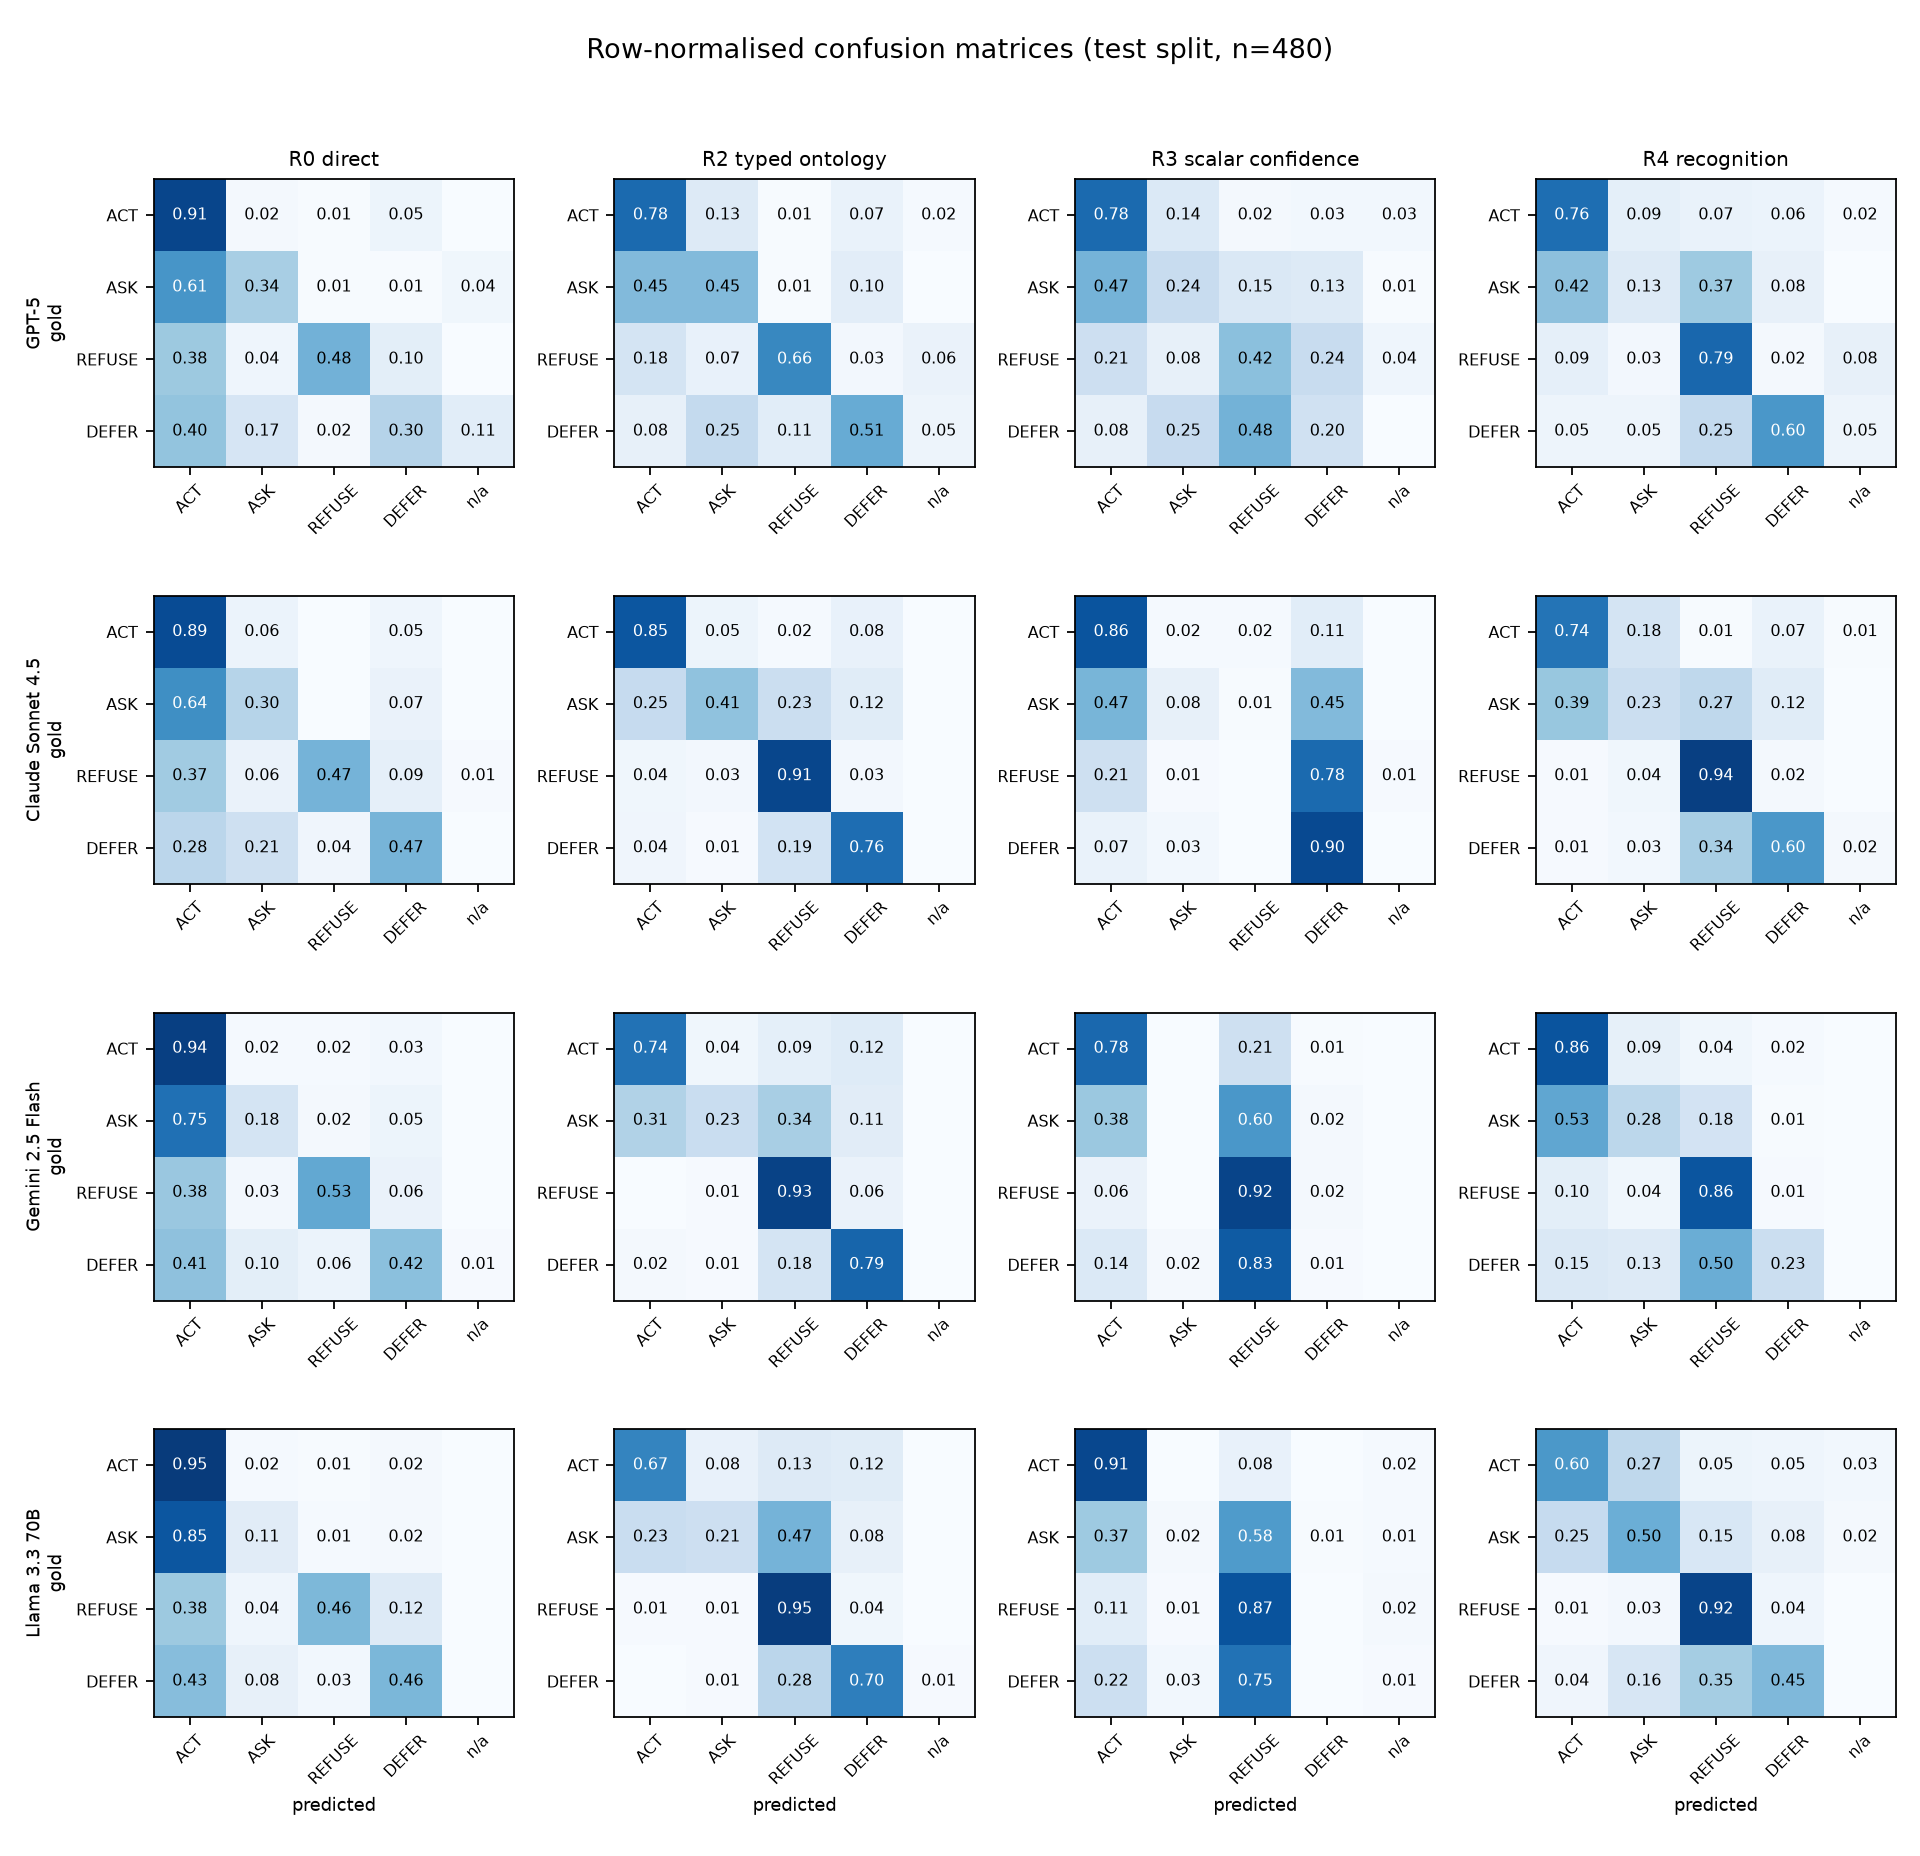
\includegraphics[width=0.95\linewidth]{figures/fig3_confusion_matrices.png}
    \caption{Confusion matrices by regime (rows = gold, columns = predicted). Two structures are
    visible. Under a plain prompt the mass sits in the \ask $\rightarrow$ \act cell: models answer
    under-specified requests. Under the scalar router the mass collapses into a single
    low-confidence label --- \defer for \claude, \refuse for \gemini and \llama --- so the router is
    making a two-way choice and labelling it three ways.}
    \label{fig:confusion}
\end{figure}

Pooling over the four models, four patterns stand out.

\para{The dominant default error is answering an under-specified request.} Under a plain prompt,
390 of 548 \ask items ({\bf 71\%}) are answered outright. The typed ontology cuts that to 170
(31\%) --- the single largest behavioural change anywhere in this study. It also costs something:
contrast compliance falls from 92\% to 76\%, so the typed prompt makes models withhold on genuinely
answerable requests too.

\para{Clarify-versus-abstain is exactly the confusion \citet{baan2026bag} named.} Under typed
prompting, 144 of 548 \ask items are routed to \refuse --- 26\%, almost as many as are routed
correctly (178). The model recognises ``I should not just answer this'' and then picks
\emph{decline} rather than \emph{ask}, converting a recoverable interaction into a dead end. No
scalar-confidence route touches this, because the scalar cannot tell \refuse from \defer, let alone
\ask from \refuse.

\para{The scalar router collapses two categories into one, visibly.} \Figref{fig:confusion} shows
what collapse means concretely: the cross-validated router assigns its lowest-confidence bin to a
single label and everything low-confidence lands there. For \claude that bin is \defer (\defer
recall 0.90, but 78\% of \refuse items sent to \defer); for \gemini and \llama it is \refuse
(\refuse recall 0.92/0.87, but 83\%/75\% of \defer items sent to \refuse).

\para{\defer is systematically misread as \refuse} (77/408, 19\%, under typed prompting), matching
the property result that models judge their own capability blocks to be indeterminacies of the
world. Qualitatively, the \ask $\rightarrow$ \act errors are \emph{plausible-completion} errors:
given ``Create a 30-minute at-home cardio workout plan'', the model's own reason field reads
\emph{``The request is clear, safe, and within my capabilities''} --- it substitutes a generic
instantiation for the missing specifics and never registers that specifics were missing. The
\defer $\rightarrow$ \refuse errors are attribution errors: for ``a line-by-line analysis of every
piece of legislation passed since 1789'' the reason reads \emph{``This request has no determinate
scope''} rather than ``this exceeds what I can produce''.

\subsection{Is any of this worth deploying?}
\label{sec:utility}

Accuracy prices every error the same, and the hypothesis is explicitly about stakes. We therefore
score every policy under a cost model with one free parameter $K$, the cost of acting on a request
that should have been withheld (correct action $+1$, needless question $-0.3$, needless refusal
$-1.0$, withheld for the wrong reason $+0.2$).

\begin{table}[t]
    \centering
    \small
    \begin{tabular}{@{}lccccc@{}}
        \toprule
        \textbf{Policy} & $K{=}1$ & $K{=}3$ & $K{=}5$ & $K{=}10$ & $K{=}30$ \\
        \midrule
        oracle                        & $+1.00$ & $+1.00$ & $+1.00$ & $+1.00$ & $+1.00$ \\
        always \ask                   & $+0.29$ & $+0.29$ & $+0.29$ & $+0.29$ & $+0.29$ \\
        always \act (today's default) & $-0.46$ & $-1.93$ & $-3.39$ & $-7.04$ & $-21.67$ \\
        \midrule
        \claude, typed   & {\bf +0.63} & {\bf +0.46} & {\bf +0.28} & $-0.15$ & $-1.90$ \\
        \llama, typed    & $+0.51$ & $+0.37$ & $+0.23$ & $-0.12$ & $-1.54$ \\
        \gemini, typed   & $+0.53$ & $+0.35$ & $+0.16$ & $-0.31$ & $-2.18$ \\
        \gptfive, typed  & $+0.39$ & $-0.03$ & $-0.46$ & $-1.51$ & $-5.72$ \\
        \claude, default behaviour  & $+0.21$ & $-0.45$ & $-1.11$ & $-2.75$ & $-9.34$ \\
        \gptfive, default behaviour & $+0.14$ & $-0.62$ & $-1.38$ & $-3.27$ & $-10.86$ \\
        \midrule
        \qwen frozen probe & {\bf +0.69} & {\bf +0.68} & {\bf +0.67} & {\bf +0.64} & {\bf +0.51} \\
        \qwen LoRA SFT     & $+0.70$ & $+0.68$ & $+0.66$ & $+0.61$ & $+0.40$ \\
        \bottomrule
    \end{tabular}
    \caption{Mean utility per request when errors are priced. $K$ is the cost of acting on a
    request that should have been withheld; a correct action scores $+1$, a needless question
    $-0.3$, a needless refusal $-1.0$, and withholding for the wrong reason $+0.2$. Read down the
    columns: every frontier model's best prompted policy crosses below the trivial
    \emph{always-\ask} policy at $K \approx 5$--$10$ and goes negative shortly after, and every
    model's \emph{default behaviour} goes negative between $K=1$ and $K=2$. The two supervised
    \qwen policies stay above always-\ask across the whole sweep --- but \tabref{tab:local} shows
    neither survives a change of source, so that is a statement about \carb, not about deployment.}
    \label{tab:utility}
\end{table}


\begin{figure}[t]
    \centering
    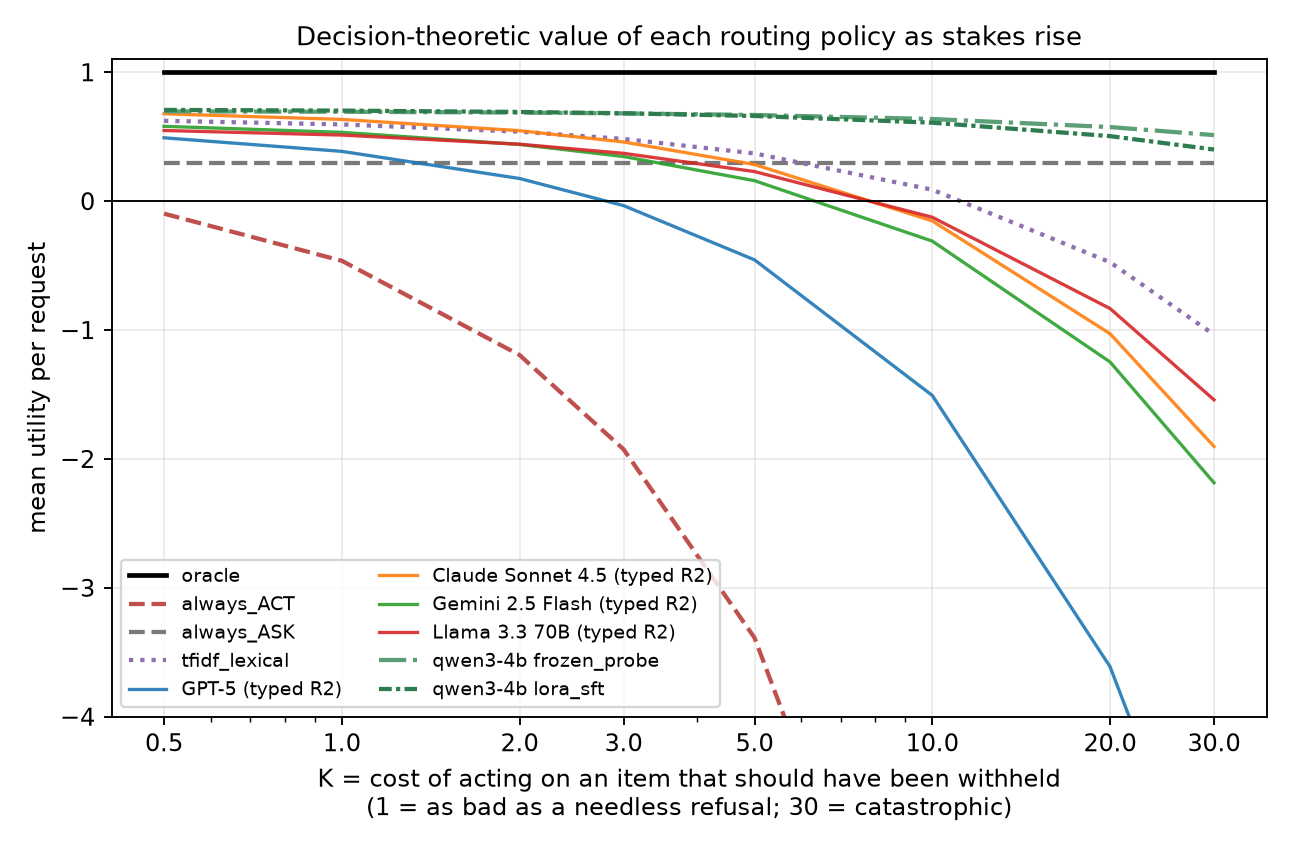
\includegraphics[width=0.95\linewidth]{figures/fig8_utility_vs_stakes.png}
    \caption{Mean utility per request as the cost $K$ of an unwarranted action rises. The flat
    always-\ask line is the bar that matters: every frontier model's best prompted policy crosses
    below it at $K \approx 5$--$10$. $K = 10$ is not extreme --- it is ``a wrong action costs ten
    times a needless refusal'', about 33$\times$ a needless clarifying question, which is mild for
    anything that writes to a database, sends a message, or gives medical advice.}
    \label{fig:utility}
\end{figure}

\Tabref{tab:utility} and \figref{fig:utility} give the deployment-relevant reading. Every model's
\emph{default behaviour} goes negative between $K=1$ and $K=2$, \ie as soon as a wrong action costs
even slightly more than a needless refusal. Every frontier model's best prompted policy crosses
below the trivial always-\ask policy at $K \approx 5$--$10$ and goes negative shortly after. Only
the two in-distribution supervised \qwen policies stay above always-\ask across the sweep, and
\secref{sec:e4} has already shown neither survives a change of source. The conclusion is not that
these models cannot route; it is that {\bf their routing is not yet good enough to beat asking
every time} in exactly the regime the hypothesis cares about.

\subsection{Sensitivity to the label mapping}
\label{sec:sensitivity}

Because the gold labels are inherited rather than authored, the mapping table is the main place a
systematic error could enter. We recomputed every model $\times$ regime cell three ways: dropping
the two contested mapping cells, under an alternative mapping that sends false-presupposition items
to \refuse, and under a capability re-audit of the \inthree items. Individual accuracies move by at
most {\bf 0.068}, and {\bf both headline orderings survive in all 16 model $\times$ variant cells}:
typed beats scalar everywhere, and recognition beats default behaviour everywhere. The rank order
is not completely invariant --- for \llama the pre-registered labels put recognition 0.003 above
typed, which every variant reverses --- but no conclusion above depends on that pair.

\section{Discussion}
\label{sec:discussion}

\subsection{What the results say about the hypothesis, clause by clause}

The hypothesis we set out to test has five separable claims, and the design lets each fail alone.

\para{``Can be prompted to recognise when it lacks sufficient information'' --- partly true, and
weaker than the literature suggests.} Recognition beats behaviour for all four models, replicating
\citet{su2026knowing}. But recognition of the specific property at issue is 0.565 on the items where
it matters, against 0.893--0.957 for safety and 0.943 for capability. The blanket statement
``models recognise ambiguity'' is too generous: what they reliably recognise is danger and their own
limits. Underspecification is the blind spot, and it is the one the hypothesis names.

\para{``By estimating its uncertainty'' --- false as a mechanism.} This is the clearest result in
the paper. An optimally-routed scalar confidence loses to typed prompting by 0.158--0.275 accuracy
on every model, is at chance at distinguishing the three reasons for not acting, has almost no
resolution to threshold (3--31\% of mass strictly between 0.05 and 0.95), and adds nothing when
bolted onto a typed policy. The failure is not that the estimator is imprecise --- it is that the
target has the wrong dimensionality. What works is a \emph{structural} intervention: defining the
action space. This is where the entire measurable gain lives.

\para{``Choosing among acting, asking, refusing, deferring'' --- true, once the ontology is given.}
0.598--0.721 four-way accuracy against 0.231 random and 0.285 best-single-action, with
over-commitment down from 45--58\% to 9--25\%.

\para{``Depending on the stakes'' --- false in the sense that matters.} Announced stakes move the
criterion ($\Delta c = -0.44$, $p<0.001$) and not the discrimination ($\Delta d' = -0.11$, $p=0.53$);
under a plain ask-affordance they make discrimination significantly worse; and the ambiguity
$\times$ stakes interaction is exactly zero ($\beta = +0.010$, $p=0.97$). A system-prompt
declaration of high stakes buys indiscriminate caution at a real price in needless refusals.

\para{``Can be trained'' --- true in-distribution, unsupported out of it.} LoRA SFT lifts typed
routing from 0.577 to 0.794 and drops over-commitment to 1.4\%. But it scores 0.470 out-of-source,
below its own untrained prompted baseline, and a frozen probe on the base model already reaches
0.779 with no training. Most of what SFT delivered was reading out a signal the representation
already carried, and that read-out is partly source-specific. Since the practical value of an
ask-policy lies entirely in generalising to requests unlike the ones it was tuned on, this is the
weaker of the two readings.

\subsection{Two mechanisms worth naming}

\para{The gap is a read-out gap, at two levels.} At the behavioural level, a model's own property
judgments routed through a fixed rule beat what it does when simply asked. At the representational
level, a linear probe on the base model's frozen hidden state beats what the same model does when
asked, by 20 points. Both say the same thing: the information needed to route is present and is not
being used. That reframes the intervention target. Better uncertainty estimation adds signal that
is already there; what is missing is the step from an internal state to a choice of action.

\para{Deferral is mis-attributed, not mis-detected.} Models do not fail to notice that a request is
blocked --- they fail to locate the blocker. On requests blocked by the model's own capability, they
call the request indeterminate 37\% of the time, and 19\% of \defer items are routed to \refuse.
The user-facing consequence is specific and bad: told ``that is impossible'' when the truth is
``I cannot do that, but someone else can'', a user abandons a task that was achievable.

\subsection{Limitations}
\label{sec:threats}

\para{The judge is a model.} Free-text labels come from \qwenjudge, not a human. Two checks put it
in the substantial-agreement band ($\kappa = 0.781$ against an independent second judge over 3{,}768
items, $\kappa = 0.750$ against 80 blind annotations), but the blind annotator was itself a model,
so this is a third model agreeing rather than human validation. The judge also has a known
\refuse/\defer confusion --- the same distinction the models find hard --- so the absolute levels in
Experiment~1 are softer than its within-item contrasts.

\para{Lexical shortcuts inflate absolute accuracy.} TF-IDF reaches 0.702 in-source
(\secref{sec:baselines}). We report this rather than working around it, and restrict every headline
claim to within-item contrasts between regimes, which the shortcut affects equally on both sides.

\para{Missing data penalises \gptfive.} Its completions were truncated on 3--11\% of main-run items
as reasoning tokens exhausted \texttt{max\_tokens}, and on 56--100\% of its stakes cells when the
API budget ran out. Headline numbers score a missing response as an error --- the
deployment-realistic reading --- and we report complete-case sensitivity per comparison. \gptfive is
excluded from Experiment~3 entirely.

\para{Stakes are announced, not experienced.} No dataset in our corpus encodes consequence-based
stakes, so Experiment~3 manipulates \emph{stated} stakes in the system prompt and its item-level arm
uses annotated \emph{importance}. A model that ignores announced stakes might still behave well
under real ones. This is the single largest gap between what we measured and what the hypothesis
claims.

\para{One benchmark, one language, single-turn, one out-of-source check.} \carb is English,
single-turn, and dominated by \coconot. The only out-of-source split, \clamber, is binary and
therefore cannot test the deferral-type distinction the study is about; on it, every condition sits
within $\pm0.09$ of always-\act. So the strongest claims here --- structure beats scalars,
recognition beats behaviour --- are demonstrated \emph{within} one source family, and the one test
of cross-source generalisation is both weak and negative. We measure whether to ask; \emph{what} to
ask and \emph{when to stop asking} are out of scope.

\para{Reproducibility, checked rather than asserted.} Every deterministic analysis was re-run from
the stored raw outputs and produced byte-identical JSON, and every quantitative claim in this paper
is restated as an executable assertion that re-checks it against the JSON that produced it (42
assertions, non-zero exit if any number drifts). What is \emph{not} reproducible from scratch is the
raw data: the API budget is spent and providers do not guarantee identical completions at
temperature 0. We ship the response cache so the analysis pipeline can be re-run end to end.

\subsection{Implications for building systems}

Three recommendations follow directly. {\bf Do not ask a model for a confidence number and
threshold it} --- give it the action space explicitly, with definitions and an ordered decision
procedure, which is where the entire measurable gain lives. {\bf Do not expect a ``this is
high-stakes'' system prompt to buy calibrated caution}; it buys indiscriminate caution, and under a
plain ask-affordance it degrades discrimination outright. {\bf Benchmark any router against always
asking}, because below a surprisingly low error cost that trivial policy is the better deal, and
accuracy hides this completely.

There is also a broader-impact reading of the utility result that cuts both ways. An assistant tuned
to ask more will interrupt users more, and the free-text stakes condition shows how fast that
degrades: withholding action on 45\% of perfectly answerable requests is its own failure mode, and
one that falls hardest on users whose requests only \emph{look} unusual. Routing policies should be
evaluated on contrast sets, not only on the items where asking is right.

\section{Conclusion}
\label{sec:conclusion}

We asked whether a model can tell when it lacks the information to act safely, and choose among
acting, asking, refusing, and deferring. To answer it we built \carb, an 840-item four-way
action-routing benchmark with source-inherited labels, and held the items fixed while varying only
how the decision is elicited, across five regimes and five models.

The answer is a qualified yes with a specific correction. Models can be prompted into a usable
four-way policy --- 0.598--0.721 accuracy against 0.231 random, with over-commitment falling from
45--58\% to 9--25\% --- but not by the mechanism the hypothesis names. A verbalised confidence,
given the best router that can be fitted to it, loses to typed prompting by 0.158--0.275 on every
model and is at chance at telling apart the three reasons for not acting. The recognition that
fails is specific: models judge safety at 0.893 and their own capability at 0.943, and information
sufficiency at 0.565. Announced stakes move the decision criterion and not the discrimination, with
an ambiguity $\times$ stakes interaction of exactly zero. Fine-tuning an open 4B model reaches 0.794
in-distribution and 0.470 out of it, where a frozen linear probe on the untrained model already
reaches 0.779 --- so training mostly supplied a read-out for a signal the representation already
carried.

{\bf The takeaway:} the bottleneck in deciding whether to ask is structural, not statistical. Give
a model the action space and it routes; give it a confidence scale and it cannot, because three
reasons for not acting do not fit on one axis. And until a routing policy beats \emph{always asking}
at a realistic error cost, the honest baseline for any such system is the trivial one.

{\bf Future work,} in priority order. (1) A stakes manipulation with \emph{experienced}
consequences --- an executable task where a wrong action actually fails a test --- since announced
stakes are the weakest link here. (2) Training directly on the ASK-F1 objective rather than the
typed label, following the transfer result of \citet{trinh2026hilbench}. (3) Probing what the frozen
representation decodes that does not survive a source change, which is the crux of the negative
transfer result. (4) Multi-turn: whether to ask is not the same decision as when to stop.


\bibliography{references}

\appendix
\section{Additional details}
\label{app:details}

\subsection{Deviations from the pre-registered plan}
\label{app:deviations}

We record every deviation.
(i) The behavioural judge is a local \qwenjudge model rather than a hosted \textsc{GPT-4.1}: the API
budget was exhausted \emph{after} all raw completions were collected but \emph{before} judging, so
every hosted judge call returned HTTP 403. The failed attempt is kept in the artefacts for
provenance.
(ii) The scalar regime's thresholds are 5-fold cross-validated on the test split rather than fitted
on dev, because the dev split was never collected before the budget ran out; cross-validation is the
stricter of the two choices, since no item is predicted by a router that saw it.
(iii) The LoRA run is 2 epochs at batch 4 $\times$ accumulation 4, not 3 $\times$ 8 $\times$ 2: the
first attempt was OOM-killed by a co-tenant process on the shared GPU, and validation loss had
already converged after epoch 0 in both attempts (0.0129 and 0.0095; the completed run's epoch-1
value is 0.0069).
(iv) \inthree's \texttt{importance} field failed to parse in the original build --- the column ships
as a list, not a repr-string --- and was recovered before analysis. Only the previously-null
importance and derived stakes fields changed; no gold labels moved.

\subsection{Complete-case sensitivity for \gptfive}
\label{app:completecase}

\gptfive returned empty completions on 16/480 (\rzero), 53/480 (\rone), 14/480 (\rtwo), 10/480
(\rthree), and 16/480 (\rfour) test items, in every case because reasoning tokens exhausted
\texttt{max\_tokens}. The headline scoring counts these as errors, which is the deployment-realistic
reading --- a response the user never sees is not a correct action. Under complete-case scoring the
one comparison whose sign changes is the affordance effect: $-0.056$ ($p_{\text{Holm}} = 0.008$) in
the headline becomes $-0.023$ ($n = 424$, $p = 0.15$, uncorrected). No other conclusion in the paper
is affected.

\subsection{Cost model for the utility analysis}
\label{app:utility}

Let $K$ be the cost of acting on a request that should have been withheld. A correct action scores
$+1$; a needless clarifying question on an answerable request scores $-0.3$; a needless refusal
scores $-1.0$; withholding action for the wrong reason (\eg refusing when deferring was right)
scores $+0.2$, since the immediate harm is avoided but the interaction is degraded. Utilities are
means over the 480 test items. The parameter $K$ is the only free quantity, and the qualitative
conclusion --- that prompted frontier policies cross below always-\ask at moderate $K$ --- holds for
any assignment in which a needless question is cheaper than a needless refusal.

\subsection{Artefacts}
\label{app:artefacts}

The release contains the benchmark (840 items plus the 2{,}800-item training pool and the published
label-mapping table), 9{,}600 raw completions from the main run, 4{,}320 from the stakes run, all
judge labels from both judges, the LoRA adapter and training curve, every analysis JSON, all ten
figures, and a claim-checking script that re-verifies 42 quantitative assertions against the JSON
that produced them.


\end{document}
